\documentclass[a4paper, 12pt, oneside, BCOR1cm, toc=chapterentrywithdots]{scrbook}

% --- Encoding and Fonts ---
\usepackage[utf8]{inputenc}
\usepackage{pifont}
\usepackage{lmodern} % Optional, better default font

% --- Common Packages ---
\usepackage{float}
\usepackage{booktabs}
\usepackage{makeidx}
\usepackage[colorlinks=false]{hyperref}
\usepackage{tocbibind}
\usepackage{blindtext}
\usepackage{rotating}
\usepackage{amsmath}
\usepackage{amssymb}
\usepackage{subfigure} 
\usepackage[nohyperlinks]{acronym}
\usepackage{multicol}
\KOMAoptions{parskip=half}
\usepackage{amsmath}
\usepackage[T1]{fontenc}
\usepackage[utf8]{inputenc} % if not default
\usepackage{microtype}   % reduces overfull boxes

\usepackage{listings}
\usepackage{xcolor} 

\usepackage{tikz}
\usepackage{tabularx}
\usepackage{array}
\usepackage{makecell}

\usepackage{pgfplots}
\usepgfplotslibrary{polar}

\usepackage{graphicx}
\usetikzlibrary{arrows.meta,positioning,fit,backgrounds}

\renewcommand{\arraystretch}{1.4}
\newcommand{\cmark}{\ding{51}} % check mark
\newcommand{\xmark}{\ding{55}} % cross mark
\usepackage[numbers]{natbib}

\setcounter{secnumdepth}{3}


% --- Hyperref Setup ---
\hypersetup{
  bookmarksnumbered=true,
  hyperindex=true,
  bookmarksopen=true,
  bookmarksopenlevel=1,
  pdfborder=0 0 0
}

% --- Custom Star Symbols ---
\newcommand{\starfull}{\ding{72}}   % Full star
\newcommand{\starhalf}{\ding{73}}   % Half star
\newcommand{\starzero}{\ding{78}}   % Empty star

% --- TOC Appearance Fixes ---
\renewcommand*{\tableofcontents}{%
  \begingroup
  \tocsection
  \tocfile{\contentsname}{toc}
  \endgroup
}
\renewcommand*{\listoffigures}{%
  \begingroup
  \tocsection
  \tocfile{\listfigurename}{lof}
  \endgroup
}
\renewcommand{\listoftables}{
  \begingroup
  \tocsection
  \tocfile{\listtablename}{lot}
  \endgroup
}

\makeindex

\begin{document}

% =====================================================
% FRONTMATTER: Roman numeral page numbering
% =====================================================
\frontmatter

% -------- Title Page --------
\begin{titlepage}
  {
    \begin{center}
        \raisebox{-1ex}{\includegraphics[scale=1.4]{images/TU_Chemnitz_positiv_gruen.pdf}}\\
    \end{center}
    \vspace{0.5cm}
  }
  \begin{center}
    \LARGE{\textbf{Privacy-Preserving Source Code Vulnerability Detection and Repair using Retrieval-Augmented LLMs for Visual Studio Code}}\\
    \vspace{1cm}
    \Large{\textbf{Master Thesis}}\\ 
    \vspace{0.5cm}
    Submitted in Fulfilment of the\\
    Requirements for the Academic Degree\\
    M.Sc. Web Engineering\\
    \vspace{0.5cm}
    Dept. of Computer Science\\
    Chair of Computer Engineering
  \end{center}
  \vspace{1cm}
  Submitted by: Md Hafizur Rahman\\
  Student ID: 806286\\
  Date: 15.12.2025\\
  \vspace{0.3cm}\\
  Internal Supervisor: Abubaker Gaber M.Sc. \\
  Internal Examiner: Dr.-Ing. Sebastian Heil \\
\end{titlepage}

% -------- Abstract --------
\addchap*{Abstract}
\addcontentsline{toc}{chapter}{Abstract}

Secure coding support within the integrated development environment is increasingly demanded, as developers prefer immediate and actionable feedback during implementation rather than deferred security checks in later pipeline stages. Traditional static application security testing tools remain effective for rule-based vulnerabilities but exhibit limitations in detecting weaknesses that require semantic reasoning, cross-file context, or domain knowledge. Large Language Models (LLMs) offer new potential for vulnerability detection and automated repair suggestions; however, their adoption is constrained by inconsistent detection quality, high false-positive rates, outdated security knowledge, and significant privacy concerns when proprietary source code is processed by cloud-based services.

This thesis investigates a privacy-preserving approach to source code vulnerability detection and repair by integrating locally deployed LLMs with Retrieval-Augmented Generation (RAG) in a Visual Studio Code extension. The proposed system operates entirely on-device, ensuring zero code exfiltration while dynamically incorporating up-to-date vulnerability knowledge from curated Common Weakness Enumeration (CWE), Common Vulnerabilities and Exposures (CVE), and OWASP sources. Two operational modes are designed: a low-latency inline mode using LLM-only inference for real-time feedback, and an audit mode that combines LLM reasoning with retrieval-based context enrichment for deeper analysis.

The system is evaluated on JavaScript and TypeScript benchmarks, including Juliet, the OWASP Benchmark, and selected real-world CVE cases. Quantitative evaluation compares LLM-only and LLM+RAG configurations against established static analysis baselines using precision, recall, F1-score, latency, and resource utilization metrics. The findings indicate that RAG-enhanced local inference improves detection consistency and recall for security-critical vulnerabilities while maintaining practical latency constraints and preserving repair suggestion quality. Overall, the results demonstrate that privacy-preserving, locally deployed LLMs augmented with retrieval-based knowledge can provide effective and reproducible vulnerability detection and repair assistance within the developer workflow.

\medskip
\noindent\textbf{Keywords:} source code security, vulnerability detection, secure code repair, large language models, retrieval-augmented generation, privacy-preserving systems, Visual Studio Code



% -------- Acknowledgment --------
\chapter*{Acknowledgment}
\addcontentsline{toc}{chapter}{Acknowledgment}
I would like to express my sincere gratitude to all those who supported me throughout the completion of this Master’s thesis.

First and foremost, I am deeply grateful to my internal supervisor, \textit{Abubaker Gaber, M.Sc.}, for his continuous guidance, constructive feedback, and professional support during all phases of this work. His availability for discussion, clear recommendations, and critical insights were instrumental in shaping both the technical direction and academic quality of the thesis.

I would also like to thank the academic staff involved in the Master’s program for providing a solid theoretical foundation and an intellectually stimulating learning environment that supported my interest in this research topic.

Furthermore, I am thankful to my colleagues and peers for their general encouragement and for fostering a motivating atmosphere throughout the study program.

Finally, I would like to express my heartfelt appreciation to my family for their constant support, understanding, and encouragement throughout my academic journey. Their support played a vital role in enabling me to complete this work.

This thesis would not have been possible without the support and contributions of the individuals mentioned above, to whom I express my sincere thanks.


% -------- Task Description --------
\chapter*{Task Description}
\addcontentsline{toc}{chapter}{Task Description}
Traditional static application security testing (SAST) tools, such as Semgrep and CodeQL, are effective for detecting predefined vulnerability patterns but cannot reason about cross-file or context-dependent weaknesses. Cloud-based language model assistants provide stronger semantic analysis yet compromise data confidentiality and reproducibility because proprietary source code must leave the local environment. This thesis aims to design and evaluate a fully local, privacy-preserving secure coding assistant for Visual Studio Code that integrates large language models (LLMs) with Retrieval-Augmented Generation (RAG). All processing occurs on the developer’s machine under a strict zero-egress policy to ensure that source code and intermediate data remain confidential.

The proposed assistant combines two complementary modes: real-time inline diagnostics that deliver immediate vulnerability alerts, and asynchronous audit and question–answering modes that use offline retrieval of vulnerability information such as CWE, CVE, and OWASP entries. A modular architecture separates the LLM inference layer, the local retrieval pipeline, and the Visual Studio Code extension interface. The system enforces privacy through local embeddings, signed corpora, and network isolation, while reproducibility is achieved through deterministic decoding, version-pinned dependencies, and containerized execution. The threat model assumes local adversaries capable of attempting code exfiltration, retrieval poisoning, or prompt injection, mitigated through corpus signing, network isolation, and provenance verification.

Evaluation will be conducted on benchmark and real-world JavaScript/TypeScript 
code. The comparison will be conducted across benchmark datasets (Juliet and 
OWASP Benchmark, approximately 40–50 test cases mapped to CWE identifiers) and 
one actively maintained real-world JavaScript/TypeScript project with documented 
vulnerabilities and verified patches. If the optional SAST baseline is executed, 
Semgrep and a scoped CodeQL subset will be included for contextual comparison. 
Evaluation metrics include precision, recall, F1-score, latency, resource usage, 
privacy validation, and reproducibility, all measured under deterministic local 
execution.

% -------- TOC, List of Figures, Tables --------
\tableofcontents
\listoffigures
\listoftables

% -------- List of Abbreviations --------
\chapter*{List of Abbreviations}
\addcontentsline{toc}{chapter}{List of Abbreviations}
\begin{multicols}{2}
\begin{acronym}[Whisper] % longest acronym for spacing

% --- A ---
\acro{ACE}{Automatic Content Extraction}
\acro{ASR}{Automatic Speech Recognition}

% --- C ---
\acro{CF}{Consistency Formatting}
\acro{Claude}{Anthropic Claude Language Model}
\acro{CRF}{Conditional Random Field}

% --- E ---
\acro{EAI}{Empty Advantage Index}
\acro{ERP}{Enterprise Resource Planning}

% --- F ---
\acro{F1}{F1 Score}
\acro{FDA}{Fill-Decision Accuracy}

% --- G ---
\acro{Gemini}{Google Gemini Language Model}
\acro{GDPR}{General Data Protection Regulation}
\acro{GPU}{Graphics Processing Unit}

% --- H ---
\acro{HMM}{Hidden Markov Model}
\acro{HR}{Hallucination Rate}

% --- I ---
\acro{ISO}{International Organization for Standardization}

% --- L ---
\acro{LLM}{Large Language Model}
\acro{LKI}{Linearised Knowledge Injection}
\acro{LoRA}{Low-Rank Adaptation}

% --- M ---
\acro{MUC-4}{Message Understanding Conference 4}

% --- N ---
\acro{NER}{Named Entity Recognition}
\acro{NES}{Non-Empty Score}
\acro{NLP}{Natural Language Processing}

% --- O ---
\acro{OBS}{Overall Baseline Score}
\acro{OCR}{Optical Character Recognition}
\acro{OAuth2}{Open Authorization 2.0}
\acro{OIDC}{OpenID Connect}
\acro{ORM}{Object-Relational Mapping}

% --- R ---
\acro{RAG}{Retrieval-Augmented Generation}
\acro{RBAC}{Role-Based Access Control}

% --- S ---
\acro{SDK}{Software Development Kit}
\acro{SF1}{Soft F1 Score}
\acro{SLU}{Spoken Language Understanding}
\acro{SLURP}{Spoken Language Understanding Resource Package}
\acro{STT}{Speech-to-Text}

% --- T ---
\acro{tRPC}{TypeScript Remote Procedure Call}
\acro{T5}{Text-to-Text Transfer Transformer}

% --- W ---
\acro{Whisper}{OpenAI Whisper Speech Recognition Model}

\end{acronym}
\end{multicols}


% =====================================================
% MAINMATTER: Arabic numerals, numbered chapters
% =====================================================
\mainmatter

\chapter{Introduction}
\label{chap:introduction}
Modern software systems form the foundation of critical infrastructure, enterprise platforms, and consumer-facing applications. As software continues to increase in size, complexity, and development velocity, vulnerabilities introduced during implementation remain one of the dominant attack vectors. Empirical studies indicate that a substantial fraction of reported security flaws originate from defects introduced during the software development phase, including injection vulnerabilities, improper input validation, insecure deserialization, and flawed access control logic \cite{pearce2022copilot,fu2023llmsec}. These weaknesses persist despite widespread adoption of secure development practices and automated analysis tools.

Static Application Security Testing (SAST) tools are commonly employed to detect vulnerabilities early in the Software Development Life Cycle (SDLC). Rule-based and taint-analysis-driven analyzers provide deterministic results and are effective for well-specified vulnerability patterns. However, prior work highlights several limitations, including high false-positive rates, limited contextual and semantic reasoning, and difficulty generalizing across diverse coding styles and frameworks \cite{sheng2025survey,li2025iris}. As a result, developers frequently face large volumes of security findings that are costly to triage and may not reflect exploitable vulnerabilities.

In contemporary development workflows, security findings are often surfaced under significant time pressure. When a vulnerability is flagged, developers must interpret diagnostic output, locate the root cause, and apply an appropriate fix while preserving functional correctness. This process is cognitively demanding and error-prone, particularly for developers without specialized security expertise. Studies have shown that security warnings are frequently ignored, misinterpreted, or resolved incorrectly, reducing the practical effectiveness of traditional static analysis tools \cite{fu2023llmsec,li2025everything}.

Recent advances in Large Language Models (LLMs) have demonstrated strong capabilities in source code understanding, generation, and transformation. LLMs can reason over programming language syntax and semantics, enabling them to identify potential defects and generate candidate repair suggestions. Consequently, LLMs have attracted significant attention as potential tools for vulnerability detection and automated repair \cite{he2023safecoder,islam2024secrepair}. However, multiple empirical evaluations indicate that LLM-generated or LLM-modified code is frequently \emph{functionally correct yet insecure}, introducing subtle vulnerabilities that are difficult to detect without explicit security grounding \cite{pearce2022copilot,peng2025cweval}. This discrepancy between functional correctness and security correctness represents a fundamental challenge for applying LLMs in secure software development.

Traditional SAST tools and LLM-based approaches exhibit complementary strengths and weaknesses. Static analyzers offer deterministic behavior and clear vulnerability specifications but lack deep contextual reasoning and adaptability. In contrast, LLMs provide strong contextual understanding and flexible reasoning but lack explicit security constraints and may hallucinate insecure solutions \cite{sheng2025survey,kavian2024llmsecguard}. This tension suggests that neither approach is sufficient in isolation for reliable vulnerability detection and repair.

Retrieval-Augmented Generation (RAG) has emerged as a promising paradigm to address these limitations by grounding LLM reasoning in external security knowledge. By augmenting model prompts with retrieved vulnerability descriptions, secure coding guidelines, and historical fixes, RAG-based systems can improve detection accuracy and reasoning consistency without requiring model retraining \cite{mialon2023augmented,shi2025rescue}. Nevertheless, most existing RAG-based secure coding systems rely on cloud-hosted models or external services, raising significant privacy and confidentiality concerns. Source code often contains proprietary logic or sensitive information, making cloud-based analysis unsuitable for regulated or security-critical environments \cite{kaur2025cyberreview,gholami2024llmcyber}.

These concerns motivate the development of privacy-preserving, locally deployed LLM systems integrated directly into the Integrated Development Environment (IDE). Local deployment enables developers to benefit from advanced reasoning capabilities while preserving code confidentiality, reducing data leakage risks, and improving reproducibility. Despite increasing interest, the design and systematic evaluation of such systems—particularly those combining retrieval, static analysis, and LLM-based reasoning within the IDE—remain underexplored \cite{basic2025slr}.

This thesis addresses this gap by investigating a privacy-preserving vulnerability detection and repair system based on retrieval-augmented local LLMs integrated into Visual Studio Code. The proposed approach combines (i) a locally hosted LLM, (ii) a curated vulnerability knowledge base, and (iii) IDE-level context extraction to support real-time detection and repair suggestions for JavaScript and TypeScript codebases. The system is evaluated against established rule-based SAST tools using reproducible benchmarks and quantitative metrics, including precision, recall, F1-score, latency, and resource usage.


\chapter{Analysis}
\label{chap:analysis}
This chapter analyzes the problem space of automated vulnerability detection and repair within modern software development workflows. The objective is to identify the fundamental technical and practical requirements for integrating Large Language Models (LLMs) into secure coding assistance, to critically examine existing approaches, and to derive design implications for a privacy-preserving, retrieval-augmented framework integrated into an Integrated Development Environment (IDE).


\section{Requirements}
\label{sec:requirements}

This section outlines the core requirements that a system must fulfill to support effective, privacy-preserving vulnerability detection and repair within modern software development workflows. The focus of this thesis is on assisting developers during implementation by identifying security-relevant weaknesses in source code and providing actionable repair suggestions directly within the Integrated Development Environment (IDE).

The primary goal of the system proposed in this thesis is to enable developers to detect and remediate vulnerabilities in JavaScript and TypeScript code using a locally deployed Large Language Model (LLM) augmented with retrieval-based security knowledge. Rather than relying on cloud-hosted services or post hoc pipeline analysis, the system operates entirely on the developer’s machine and integrates seamlessly into Visual Studio Code. Source code, analysis results, and vulnerability knowledge remain local at all times, ensuring privacy, reproducibility, and suitability for regulated or security-sensitive environments.

In contrast to traditional Static Application Security Testing (SAST) tools, which rely on predefined rules and often provide limited remediation guidance, the proposed system leverages LLM-based semantic reasoning combined with Retrieval-Augmented Generation (RAG). This enables the system to reason about code context, explain detected issues, and suggest concrete repairs grounded in curated vulnerability knowledge. To ensure practical usefulness, the system must satisfy both functional and non-functional requirements related to accuracy, transparency, performance, and usability.

Based on the challenges identified in Chapter~\ref{chap:introduction} and the analysis of existing approaches, six core requirements (R1–R6) are defined. These requirements establish a systematic basis for evaluating the proposed architecture and guide the design decisions discussed in subsequent chapters.

\textbf{R1 – Detection Accuracy and Consistency:}  
The system must reliably identify security-relevant vulnerabilities in source code with stable behavior across repeated analyses. Detection results should be consistent for identical inputs, independent of invocation timing or interaction mode. The system should minimize false positives while maintaining adequate recall, ensuring that developers can trust reported findings and are not overwhelmed by spurious warnings.

\textbf{R2 – Context-Aware Vulnerability Reasoning:}  
The system must analyze vulnerabilities in their surrounding code context rather than relying solely on syntactic patterns. This includes reasoning about data flow, API usage, and control structures at the function and file level. The system should correctly distinguish between vulnerable and benign code patterns that appear syntactically similar and must avoid flagging issues that are mitigated by contextual safeguards.

\textbf{R3 – Explainability and Transparency:}  
To foster developer trust and facilitate efficient remediation, the system must provide transparent explanations for detected vulnerabilities. Each finding should be accompanied by a clear description of the underlying weakness, references to relevant vulnerability classes (e.g., CWE), and an indication of which code fragments contributed to the detection. Explanations should be concise, technically precise, and suitable for developers without specialized security expertise.

\textbf{R4 – Actionable Repair Suggestions:}  
The system must generate concrete, security-aware repair suggestions that address the root cause of detected vulnerabilities while preserving functional correctness. Suggested fixes should be directly applicable to the affected code region and must avoid introducing new security issues or breaking existing behavior. Developers must retain full control over whether and how suggested changes are applied.

\textbf{R5 – Privacy-Preserving Operation:}  
All analysis, retrieval, and generation steps must be performed locally without transmitting source code or derived artifacts to external services. The system must operate with locally deployed models and locally stored vulnerability knowledge, ensuring that proprietary code remains confidential and that results are reproducible across environments.

\textbf{R6 – Usability and Responsiveness:}  
The system must integrate smoothly into the IDE and provide feedback within acceptable latency bounds. Inline detection should support near–real-time interaction to avoid disrupting the development flow, while more comprehensive audit operations may tolerate higher latency. Usability is evaluated with respect to end-to-end response time, clarity of presented information, and compatibility with typical developer hardware configurations.

These six requirements define the evaluation criteria for the proposed system. In the following chapters, each requirement is addressed through specific architectural choices and implementation strategies. The evaluation chapter assesses to what extent the system satisfies these requirements in practice, using quantitative metrics and reproducible benchmarks.

\subsection{R1: Detection Accuracy and Consistency}\vspace{-2mm}

\label{sec:r1-consistency}

Consistency refers to the system’s ability to produce stable, repeatable, and uniformly structured vulnerability detection results when analyzing identical or semantically equivalent source code. In the context of security analysis, consistency means that the same vulnerability is detected, classified, explained, and localized in a comparable manner across repeated runs, invocation modes, and interaction contexts.

Unlike general-purpose code analysis, vulnerability detection demands a high degree of determinism. Security findings are often used to guide remediation decisions, trigger audits, or satisfy compliance requirements. Inconsistent detection outcomes—such as reporting a vulnerability in one analysis but not in another, or fluctuating between different vulnerability classes—undermine developer trust and reduce the practical usability of the system. More generally, LLM-based systems are known to exhibit non-deterministic behavior and hallucination under unconstrained generation, motivating strict prompting and grounding strategies for stable outputs \cite{openai2023gpt4,ji2023hallucination,pearce2022copilot}.

% As illustrated in Figure~\ref{fig:ide-detection-example}, an
An ideal solution should ensure that once a vulnerability is identified, it is reported in a consistent manner. This includes stable classification (e.g., mapping to the same CWE category), consistent localization of the affected code region, and uniform explanation structure. For example, an input validation flaw should not alternately be reported as a generic "security issue," an injection vulnerability, or a logic error across different executions if the underlying code has not changed.

Consistency operates across multiple dimensions of vulnerability reporting. At the level of detection outcome, the presence or absence of a vulnerability should be stable across repeated analyses. At the level of classification, detected issues should map consistently to the same vulnerability categories and severity levels. At the level of explanation, descriptions should follow standardized phrasing and structure, avoiding unnecessary variation in terminology or level of detail. At the level of localization, the same code regions should be highlighted as relevant to the vulnerability.

This requirement is particularly critical because modern development workflows increasingly rely on automated security feedback integrated into the IDE. If a vulnerability warning appears intermittently or changes classification without code modifications, developers may disregard the warning entirely. Similar concerns have been documented in studies of static analysis tools, where inconsistent or noisy warnings reduce adoption and remediation rates \cite{johnson2013don}.

From a system design perspective, achieving consistency requires controlling sources of nondeterminism in LLM inference and grounding vulnerability reasoning in structured security knowledge. Retrieval-Augmented Generation contributes to this goal by anchoring model outputs to curated vulnerability descriptions and examples, thereby reducing reliance on purely generative reasoning and mitigating hallucination.

For evaluation, detection consistency is assessed using repeated analyses of identical code samples under fixed configurations. We measure agreement between runs using macro-averaged precision, recall, and F1-score for vulnerability presence and classification. In addition, label agreement metrics are used to quantify stability in vulnerability categorization across runs. A high degree of agreement indicates that the system produces stable and reliable security findings.

\begin{table}[h!]
\centering
\renewcommand{\arraystretch}{1.6}
\setlength{\tabcolsep}{12pt}
\begin{tabularx}{\textwidth}{|>{\centering\arraybackslash}m{3cm}|>{\arraybackslash}X|}
\hline
\textbf{Consistency Level} & \textbf{Interpretation (example thresholds)} \\
\hline
High &
\textbf{High consistency.} Vulnerability presence and classification are stable across runs (macro F1 $\geq 0.80$), with minimal variation in localization and explanation structure. \\
\hline
Medium &
\textbf{Moderate consistency.} Minor variations in classification or explanation occur (macro F1 in $[0.65, 0.80)$), but core vulnerability detection remains stable. \\
\hline
Low &
\textbf{Low consistency.} Frequent changes in vulnerability presence or classification (macro F1 in $[0.50, 0.65)$), indicating unstable detection behavior. \\
\hline
None &
\textbf{No consistency.} Detection results vary substantially across runs (macro F1 $< 0.50$), undermining trust in the system. \\
\hline
\end{tabularx}
\caption{Evaluation scale for R1: Detection Consistency (example thresholds).}
\label{tab:r1-detection-consistency}
\end{table}

In summary, R1 ensures that vulnerability detection results are stable, reproducible, and uniformly structured across repeated analyses. By enforcing consistency across detection outcomes, classification, explanation, and localization, the system provides developers with reliable security feedback that can be trusted and acted upon within real-world development workflows.
 

\subsection{R2: Context-Aware Vulnerability Reasoning}\vspace{-2mm}
\label{sec:r2-context-awareness}

Context-aware vulnerability reasoning refers to the system's ability to correctly identify, classify, and localize security vulnerabilities by analyzing source code within its surrounding semantic and structural context. This requirement goes beyond surface-level pattern matching and instead relies on understanding data flow, control flow, API semantics, and usage constraints to determine whether a code fragment constitutes a genuine security risk.

In contrast to traditional static analyzers that operate primarily on syntactic rules or predefined patterns, effective vulnerability reasoning must consider how code behaves in context. Prior research has shown that many vulnerabilities only manifest under specific execution paths, input assumptions, or API usage scenarios, and cannot be reliably detected without contextual analysis \cite{livshits2005java,chess2004staticanalysis}. Similarly, LLM-based approaches that lack explicit grounding may misclassify benign code as vulnerable or overlook subtle security flaws when context is incomplete or fragmented \cite{pearce2022copilot,ji2023hallucination}.

% As illustrated in Figure~\ref{fig:ide-detection-example}, an
An ideal solution must detect vulnerabilities even when relevant information is distributed across multiple statements, functions, or files. The system should associate related code fragments into a coherent reasoning context while ignoring unrelated logic. For example, input validation performed in a helper function should be correctly recognized when assessing the safety of downstream API usage, and defensive checks should prevent false positives when they effectively mitigate a potential vulnerability.

This requirement is critical because real-world codebases are rarely self-contained or linear. Security-relevant information is often scattered across variable initializations, conditional branches, utility functions, and framework abstractions. Without robust contextual reasoning, a system may either miss vulnerabilities that emerge from interdependent logic or incorrectly flag code that is secure by design. Such errors reduce developer confidence and limit the system’s usefulness in practice.

Effective context-aware reasoning operates along three complementary dimensions. First, the system must correctly integrate dispersed information. Security-relevant signals may appear in different parts of a file or across multiple files, and the system must combine these fragments into a unified vulnerability assessment. Second, the system must recognize mitigation logic. If appropriate safeguards—such as input sanitization, authentication checks, or bounds validation—are present, the system should account for them and avoid reporting false positives. Third, the system must avoid unsupported inference. When insufficient context is available to determine whether a vulnerability exists, the system should explicitly acknowledge uncertainty rather than hallucinating a definitive conclusion.

Retrieval-Augmented Generation supports this requirement by grounding vulnerability reasoning in structured security knowledge, such as Common Weakness Enumeration (CWE) descriptions, secure coding guidelines, and historical vulnerability examples. Retrieved context helps the model align observed code patterns with known vulnerability semantics, reducing reliance on implicit assumptions and improving reasoning reliability.

The advantages of strong context-aware vulnerability reasoning are multifold. It improves detection accuracy by reducing false positives and false negatives caused by superficial pattern matching. It enhances robustness to coding style variation by focusing on semantic behavior rather than syntactic form. It also improves developer trust, as reported vulnerabilities more closely align with actual security risks in the codebase.

For evaluation, context-aware reasoning is assessed using classification metrics that measure the correctness of vulnerability detection and categorization in context-rich scenarios. Precision, recall, and macro-averaged F1-score are computed over benchmarks containing both vulnerable and non-vulnerable code samples with similar surface patterns. In addition, localization accuracy is measured by evaluating whether the system correctly identifies the relevant code regions contributing to the vulnerability. These metrics collectively capture the system’s ability to reason about vulnerabilities in context rather than in isolation.

\begin{table}[h!]
\centering
\renewcommand{\arraystretch}{1.6}
\setlength{\tabcolsep}{12pt}
\begin{tabularx}{\textwidth}{|>{\centering\arraybackslash}m{3cm}|>{\arraybackslash}X|}
\hline
\textbf{Reasoning Level} & \textbf{Interpretation (example criteria)} \\
\hline
High &
\textbf{High context awareness.} The system correctly integrates dispersed context, recognizes mitigation logic, and avoids unsupported inference. Vulnerability classification and localization are accurate (macro F1 $\geq 0.80$). \\
\hline
Medium &
\textbf{Moderate context awareness.} The system integrates some contextual information but occasionally misses mitigations or misinterprets dependencies (macro F1 in $[0.65, 0.80)$). \\
\hline
Low &
\textbf{Low context awareness.} The system relies primarily on surface patterns, leading to frequent false positives or missed vulnerabilities (macro F1 in $[0.50, 0.65)$). \\
\hline
None &
\textbf{No context awareness.} The system fails to incorporate contextual information and produces unreliable vulnerability assessments (macro F1 $< 0.50$). \\
\hline
\end{tabularx}
\caption{Evaluation scale for R2: Context-Aware Vulnerability Reasoning.}
\label{tab:r2-context-awareness}
\end{table}

In summary, R2 ensures that vulnerability detection is grounded in semantic and structural understanding of source code rather than superficial pattern matching. By integrating dispersed context, accounting for mitigation logic, and avoiding unsupported assumptions, the system provides accurate and trustworthy vulnerability assessments that reflect real-world security risks in modern codebases.


\subsection{R3: Explainability and Transparency}\vspace{-2mm}
\label{sec:r3-transparency}

Explainability and transparency refer to the system's ability to make its vulnerability detection and repair reasoning understandable, inspectable, and verifiable by developers. In the context of security analysis, transparency means that the system does not merely report that a vulnerability exists, but clearly communicates \emph{why} it was detected, \emph{which code elements contributed to the decision}, and \emph{what security principles are being violated}. This requirement is essential for fostering developer trust, enabling informed remediation decisions, and supporting auditability in security-sensitive environments.

Unlike traditional static analyzers, which often expose explicit rules or taint paths, LLM-based systems risk operating as opaque black boxes. Prior research has shown that when developers cannot understand the rationale behind automated security findings, they are more likely to ignore warnings or apply fixes incorrectly \cite{johnson2013don, christakis2016developers}. This issue is amplified for LLM-based approaches, where probabilistic reasoning and generative explanations may obscure the causal relationship between code patterns and reported vulnerabilities.

% As illustrated in Figure~\ref{fig:ide-detection-example}, an
An ideal solution should present vulnerability findings alongside structured explanations that link detected issues to concrete code regions and recognized vulnerability classes. For example, when reporting an injection vulnerability, the system should indicate the untrusted input source, the absence or insufficiency of validation or sanitization, and the sensitive sink where exploitation may occur. Explanations should be concise, technically precise, and aligned with established security taxonomies such as the Common Weakness Enumeration (CWE).

Explainability operates across several dimensions. At the level of localization, the system should highlight the specific lines or code fragments that contributed to the detection, enabling developers to quickly identify the relevant context. At the level of reasoning, the system should describe the logical chain that led from observed code patterns to the vulnerability conclusion, avoiding vague or purely descriptive statements. At the level of justification, the system should reference recognized vulnerability categories or security guidelines to ground its explanations in established knowledge rather than ad hoc model intuition.

This requirement is particularly important in real-world development workflows, where developers must often balance security concerns against functional requirements and delivery timelines. Transparent explanations allow developers to assess whether a reported issue is relevant in their specific context and to determine whether a suggested fix aligns with project constraints. In regulated domains, transparency further supports accountability by enabling security findings to be reviewed, documented, and justified during audits.

Retrieval-Augmented Generation plays a central role in supporting explainability. By grounding explanations in retrieved vulnerability descriptions, secure coding guidelines, and historical examples, the system can produce explanations that are both informative and consistent. This reduces the risk of hallucinated or misleading justifications and improves alignment between detection outcomes and established security knowledge.

For evaluation, explainability and transparency are assessed through a combination of qualitative and quantitative criteria. We evaluate whether explanations correctly reference the underlying vulnerability type, accurately identify the contributing code regions, and maintain internal coherence between detection, explanation, and suggested repair. In addition, explanation completeness is assessed by verifying that all essential components of the vulnerability reasoning—such as source, sink, and missing mitigation—are explicitly addressed. While explainability is inherently qualitative, structured scoring rubrics enable reproducible assessment across benchmarks.

\begin{table}[h!]
\centering
\renewcommand{\arraystretch}{1.6}
\setlength{\tabcolsep}{12pt}
\begin{tabularx}{\textwidth}{|>{\centering\arraybackslash}m{3cm}|>{\arraybackslash}X|}
\hline
\textbf{Transparency Level} & \textbf{Interpretation (example criteria)} \\
\hline
High &
\textbf{High transparency.} Explanations clearly identify the vulnerability type, affected code regions, and reasoning steps, and reference established security knowledge. Developers can easily verify and act on the findings. \\
\hline
Medium &
\textbf{Moderate transparency.} Explanations identify the vulnerability and affected code but provide limited reasoning detail or incomplete justification. Additional developer interpretation is required. \\
\hline
Low &
\textbf{Low transparency.} Explanations are vague, generic, or loosely connected to the reported vulnerability, making verification difficult. \\
\hline
None &
\textbf{No transparency.} The system reports vulnerabilities without meaningful explanation or justification, effectively operating as a black box. \\
\hline
\end{tabularx}
\caption{Evaluation scale for R3: Explainability and Transparency.}
\label{tab:r3-transparency}
\end{table}

R3 ensures that findings are understandable and reviewable, not just correct in aggregate metrics. Clear links between code evidence, vulnerability class, and suggested action are necessary for developer trust and accountable use.


\subsection{R4: Actionable Repair Suggestions}\vspace{-2mm}
\label{sec:r4-repair-quality}

Actionable repair suggestions refer to the system's ability to generate concrete, security-aware code modifications that effectively remediate detected vulnerabilities while preserving the original program's functional correctness. In contrast to generic advice or high-level recommendations, actionable repairs must be directly applicable to the affected code region and sufficiently specific to support immediate developer adoption.

In the context of vulnerability detection, identifying a security flaw is only the first step. Developers ultimately require guidance on how to fix the issue correctly and efficiently. Empirical evidence suggests that warning overload and unclear remediation guidance reduce adoption and follow-through, especially when developers must interpret findings and design fixes under time pressure \cite{johnson2013don,christakis2016developers}. Automated program repair research also highlights that patch quality and evaluation are non-trivial: fixes must address the root cause without introducing regressions or unintended behavior changes \cite{weimer2009genprog,kim2013par,monperrus2014critique}. Inconsistent or incorrect fixes may leave vulnerabilities partially unresolved or introduce new flaws, undermining the value of automated detection.

% As illustrated in Figure~\ref{fig:ide-repair-example}, an
An ideal solution should provide repair suggestions that are tightly coupled to the detected vulnerability and localized to the relevant code region. For example, if an injection vulnerability is identified, the system should suggest concrete input validation or parameterization mechanisms that are appropriate for the specific API and execution context, rather than issuing abstract recommendations such as "sanitize input." Suggested repairs should reflect established secure coding practices and align with recognized vulnerability classes, such as those defined by the Common Weakness Enumeration (CWE) and practitioner guidance such as OWASP cheat sheets \cite{mitreCWE,owaspCheatSheets,owaspSqlCheatSheet,owaspXssCheatSheet}.

More broadly, actionable repair guidance should cover a range of common weakness classes beyond injection, including CSRF defenses, robust input validation, safe deserialization, secure file upload handling, password storage, and security logging practices \cite{owaspCsrfCheatSheet,owaspInputValidationCheatSheet,owaspDeserializationCheatSheet,owaspFileUploadCheatSheet,owaspPasswordStorageCheatSheet,owaspLoggingCheatSheet}.

Actionable repair suggestions operate across several dimensions. At the level of specificity, suggested fixes must include precise code changes rather than vague guidance. At the level of correctness, repairs must eliminate the underlying vulnerability without breaking existing functionality or introducing new security issues. At the level of contextual appropriateness, fixes should respect the surrounding code structure, library usage, and project conventions, avoiding disruptive or unrealistic refactorings. Finally, at the level of control, developers must retain full authority over whether and how suggested repairs are applied.

This requirement is particularly important in IDE-integrated workflows, where developers expect rapid, low-friction assistance. Repair suggestions that are overly verbose, difficult to interpret, or incompatible with the existing codebase are likely to be ignored. Conversely, concise and correct fixes that can be reviewed and applied incrementally encourage adoption and improve remediation rates.

Retrieval-Augmented Generation supports actionable repair suggestions by grounding generated fixes in curated vulnerability knowledge and historical remediation examples. Retrieved context enables the system to align suggested repairs with established security practices and reduce the risk of hallucinated or insecure fixes. By decoupling security knowledge from the model parameters, RAG further allows repair logic to evolve as new vulnerability patterns and recommended mitigations emerge.

For evaluation, repair quality is assessed using a combination of functional and security-oriented metrics. Functional correctness is evaluated by verifying that repaired code preserves expected behavior, for example through regression tests or benchmark-provided test cases. Security effectiveness is evaluated by re-analyzing the repaired code to confirm that the original vulnerability is no longer detected and that no new vulnerabilities are introduced. In addition, repair precision is assessed by measuring the proportion of suggested fixes that are both applicable and correct without manual modification.

\begin{table}[h!]
\centering
\renewcommand{\arraystretch}{1.6}
\setlength{\tabcolsep}{12pt}
\begin{tabularx}{\textwidth}{|>{\centering\arraybackslash}m{3cm}|>{\arraybackslash}X|}
\hline
\textbf{Repair Quality Level} & \textbf{Interpretation (example criteria)} \\
\hline
High &
\textbf{High-quality repairs.} Suggested fixes are directly applicable, remove the vulnerability, preserve functional correctness, and align with secure coding practices. \\
\hline
Medium &
\textbf{Moderate-quality repairs.} Suggested fixes address the vulnerability but require minor manual adjustment or introduce small, non-critical side effects. \\
\hline
Low &
\textbf{Low-quality repairs.} Suggested fixes are vague, incomplete, or partially incorrect, requiring substantial developer intervention. \\
\hline
None &
\textbf{No actionable repair.} The system fails to provide a usable fix or produces insecure or functionally incorrect code. \\
\hline
\end{tabularx}
\caption{Evaluation scale for R4: Actionable Repair Suggestions.}
\label{tab:r4-repair-quality}
\end{table}

R4 bridges detection and remediation. In practice, suggestions are valuable only when they are specific, context-appropriate, and safe to review incrementally, while final control remains with the developer.


\subsection{R5: Privacy-Preserving Operation}\vspace{-2mm}
\label{sec:r5-privacy}

Privacy-preserving operation refers to the system's ability to perform vulnerability detection, reasoning, and repair generation without exposing source code or derived artifacts to external services. This requirement ensures that all stages of analysis—including model inference, retrieval of security knowledge, and generation of explanations or fixes—are executed locally within the developer's environment.

Source code frequently contains proprietary logic, intellectual property, or sensitive business information. In many industrial, governmental, and regulated settings, transmitting such data to cloud-hosted services is unacceptable due to confidentiality, compliance, or contractual constraints. Consequently, any practical vulnerability detection system intended for real-world adoption must provide strong guarantees that code remains under the developer's control at all times.

% As illustrated in Figure~\ref{fig:local-architecture-overview}, an
An ideal solution should operate entirely on local hardware, using locally deployed LLMs and locally stored vulnerability knowledge bases. No source code, intermediate representations, embeddings, or analysis results should be transmitted beyond the local machine. This includes not only raw code but also prompts, retrieved documents, and generated outputs, all of which may inadvertently leak sensitive information if handled improperly.

Privacy-preserving operation encompasses several dimensions. At the level of deployment, the system must rely exclusively on local inference engines and avoid dependencies on external APIs or remote model hosting. At the level of data handling, all inputs and outputs must remain confined to local memory or storage, with no background telemetry or logging that could result in unintended data egress. At the level of reproducibility, local execution ensures that analysis results can be replicated across environments without reliance on changing external services or opaque model updates.

This requirement is particularly important for vulnerability detection, where analysis often requires access to complete source files or project-level context. Partial redaction or anonymization strategies are insufficient, as they may remove security-relevant information and degrade detection accuracy. By contrast, local execution allows full-context analysis while maintaining strict confidentiality.

Retrieval-Augmented Generation supports privacy-preserving operation by decoupling security knowledge from the model parameters and enabling the use of locally maintained knowledge bases. Vulnerability descriptions, secure coding guidelines, and historical examples can be curated and updated locally without requiring cloud-based retrieval or retraining. This design enables timely incorporation of new vulnerability knowledge while preserving data sovereignty.

For evaluation, privacy preservation is assessed through architectural inspection and runtime verification. We verify that no network communication occurs during analysis by monitoring outbound connections and ensuring that all model inference and retrieval operations are confined to local processes. In addition, we assess whether the system functions correctly in offline environments, confirming that detection and repair capabilities do not degrade when network access is unavailable. These checks provide objective evidence that privacy guarantees are upheld in practice.

\begin{table}[h!]
\centering
\renewcommand{\arraystretch}{1.6}
\setlength{\tabcolsep}{12pt}
\begin{tabularx}{\textwidth}{|>{\centering\arraybackslash}m{3cm}|>{\arraybackslash}X|}
\hline
\textbf{Privacy Level} & \textbf{Interpretation (example criteria)} \\
\hline
High &
\textbf{Strong privacy guarantees.} All analysis stages run locally, no network communication is observed, and the system functions fully offline without loss of capability. \\
\hline
Medium &
\textbf{Partial privacy.} Core analysis is local, but auxiliary components (e.g., optional updates or logging) require network access. No source code is transmitted. \\
\hline
Low &
\textbf{Weak privacy.} Some analysis steps or prompts rely on external services, introducing potential data exposure risks. \\
\hline
None &
\textbf{No privacy guarantees.} Source code or derived artifacts are transmitted to remote services during analysis. \\
\hline
\end{tabularx}
\caption{Evaluation scale for R5: Privacy-Preserving Operation.}
\label{tab:r5-privacy}
\end{table}

In summary, R5 ensures that vulnerability detection and repair can be performed without compromising source code confidentiality. By enforcing fully local execution, eliminating external dependencies, and enabling offline operation, the system addresses a key barrier to adoption of LLM-based security assistance in real-world, security-sensitive development environments.


\subsection{R6: Usability and Responsiveness}\vspace{-2mm}
\label{sec:r6-usability}

Usability in the context of the proposed framework refers primarily to \textbf{latency}, defined as the end-to-end time delay between a developer action and the presentation of security feedback within the Integrated Development Environment (IDE). This includes the time required for context extraction, model inference, retrieval-augmented reasoning, and rendering of vulnerability findings or repair suggestions. While the system supports multiple interaction modes, the core task is the transformation of \emph{source code input} into \emph{actionable security feedback}. Accordingly, the latency requirement applies uniformly across inline detection, on-demand analysis, and repair suggestion workflows.

Responsiveness directly determines whether security assistance can be integrated naturally into the development process. Human–computer interaction research consistently shows that feedback delivered within a few seconds preserves a sense of flow and supports effective turn-taking, whereas longer delays disrupt concentration and reduce tool adoption \cite{card1991model, nielsen1994usability}. In the context of IDE-based development, developers expect near-immediate feedback comparable to other static diagnostics such as type errors or linting warnings. Excessive latency risks relegating security analysis to a background task that is ignored or deferred.

% As illustrated in Figure~\ref{fig:ide-interaction-example}, vulnerability
Vulnerability annotations and repair suggestions should appear promptly after a triggering event, such as saving a file or explicitly invoking an analysis command. Timely feedback enables developers to assess security implications while the relevant code context is still active, reducing cognitive load and improving remediation efficiency.

Unlike other requirements—such as detection accuracy (R1), contextual reasoning (R2), explainability (R3), repair quality (R4), or privacy preservation (R5)—usability in this thesis is scoped strictly to latency. This focus reflects the practical reality that even accurate and well-explained security findings are unlikely to be acted upon if they arrive too late to fit within normal development workflows. This concern is particularly relevant for local LLM-based systems, where inference time can be substantial compared to traditional static analysis.

Latency, however, is not an absolute property of the system alone. It is strongly influenced by the \textbf{hardware and deployment environment} on which the system operates. Dedicated accelerators such as GPUs can significantly reduce inference time, whereas CPU-only or resource-constrained environments typically incur higher latency. Additionally, factors such as model size, retrieval depth, and concurrency affect responsiveness. For this reason, all latency measurements must be reported together with the corresponding hardware profile, including processor type, available memory, and accelerator configuration. This ensures that usability claims are interpreted relative to realistic deployment scenarios rather than as hardware-agnostic performance guarantees.

For evaluation, usability is measured using the 95th percentile end-to-end (p95 E2E) latency across representative interaction scenarios. The p95 metric captures worst-case responsiveness experienced by users while remaining robust to isolated outliers. Separate latency measurements are reported for interactive inline detection and for more comprehensive, explicitly triggered analyses.

\begin{table}[h!]
\centering
\renewcommand{\arraystretch}{1.6}
\setlength{\tabcolsep}{12pt}
\begin{tabularx}{\textwidth}{|>{\centering\arraybackslash}m{3cm}|>{\arraybackslash}X|}
\hline
\textbf{Visual Score} & \textbf{Interpretation} \\
\hline
\centering\raisebox{0pt}{\tikz[baseline]{\filldraw[fill=black] (0,0) circle (0.4cm);}} 
& \textbf{High usability.} p95 end-to-end latency $\leq$ 2\,s for inline detection on the declared hardware profile. Interaction remains fluid and non-disruptive. \\
\hline
\centering\raisebox{0pt}{\tikz[baseline]{\filldraw[fill=black] (0,0) -- (90:0.4cm) arc (90:-90:0.4cm) -- cycle; \draw (0,0) circle (0.4cm);}}
& \textbf{Medium usability.} p95 end-to-end latency in $(2, 5)$\,s. Delay is noticeable but acceptable for security feedback that is not continuously triggered. \\
\hline
\centering\raisebox{0pt}{\tikz[baseline]{\draw (0,0) circle (0.4cm);}} 
& \textbf{No usability.} p95 end-to-end latency $>$ 5\,s for inline scenarios or frequent timeouts. Feedback is too slow for practical integration into the development workflow. \\
\hline
\end{tabularx}
\caption{Evaluation scale for R6: Usability (Latency).}
\label{tab:r6-usability}
\end{table}

In summary, usability in this framework is defined as responsiveness measured through end-to-end latency for IDE-integrated vulnerability detection and repair. Because latency is inherently dependent on hardware and deployment conditions, all usability evaluations must be contextualized by reporting the corresponding execution environment. This ensures that results are comparable, interpretable, and grounded in realistic usage scenarios.



\section{Related Work}
\label{sec:related-work}

This section reviews prior research relevant to LLM-based vulnerability detection and repair, with a focus on static analysis approaches, large language models for software security, retrieval-augmented generation, and privacy-preserving deployment. The discussion highlights both the strengths and limitations of existing work and positions the present thesis within the current research landscape.

\subsection{Traditional Static Application Security Testing}\vspace{-2mm}
Static Application Security Testing (SAST) tools have long been the primary means of detecting vulnerabilities during development. Rule-based analyzers and taint-analysis systems, such as Semgrep and CodeQL, identify predefined vulnerability patterns by statically inspecting source code \cite{semgrepDocs,codeqlDocs}. These tools provide deterministic and reproducible results, which makes them suitable for automated pipelines and compliance-driven environments.

From a research perspective, modern static analyzers build on foundational ideas such as abstract interpretation \cite{cousot1977abstract} and scalable bug-finding techniques \cite{engler2001bugs}. In practice, large-scale deployments demonstrate that static analysis can find real defects in industrial codebases at massive scale \cite{bessey2010billion}. Security-oriented static analysis has also been studied explicitly, including work that frames static analysis as an effective security engineering control when combined with secure development processes \cite{chess2004staticanalysis,howard2006sdl,mcgraw2006softwaresecurity}.

Despite these strengths, SAST tools can struggle with contextual reasoning and generalization. They frequently produce false positives when security-relevant patterns appear in benign contexts (e.g., input validated elsewhere, framework-enforced invariants) and may miss vulnerabilities that depend on semantic relationships or framework-specific behavior. Moreover, many SAST tools offer limited remediation guidance, requiring developers to interpret findings and manually design fixes. Empirical studies show that warning overload and poor actionability reduce adoption and remediation rates \cite{johnson2013don,christakis2016developers}.

These limitations motivate research into approaches that complement deterministic static analysis with more flexible reasoning and explanation generation. In this thesis, Code Guardian aims to preserve the determinism and localization benefits of IDE diagnostics while using LLM-based reasoning (grounded by security knowledge) to improve explanation quality and provide developer-controlled repair suggestions.


\subsection{LLM-Based Vulnerability Detection and Repair}\vspace{-2mm}
Recent advances in Large Language Models (LLMs) have prompted extensive investigation into their use for vulnerability detection and secure code generation. Empirical studies demonstrate that LLMs can identify security flaws and generate syntactically correct code across a range of programming tasks \cite{fu2023llmsec}. However, early evaluations reveal that LLM-generated code is often \emph{functionally correct yet insecure}, containing subtle vulnerabilities that are not immediately apparent \cite{pearce2022copilot,peng2025cweval}.

Several approaches attempt to address these shortcomings through fine-tuning or constrained decoding. SafeCoder introduces security-aware fine-tuning to bias models toward safer outputs \cite{he2023safecoder}, while constrained decoding techniques enforce security constraints during generation \cite{li2024constrained}. Although effective in controlled settings, these methods require curated training data, retraining effort, or auxiliary security models, limiting their adaptability and suitability for local, resource-constrained deployment.

Other systems combine LLMs with static analyzers to mitigate hallucinations and improve reliability. LLM Security Guard integrates static analysis feedback into LLM reasoning to strengthen vulnerability detection \cite{kavian2024llmsecguard}. Similarly, IRIS employs LLMs to assist static analysis by interpreting and refining vulnerability reports \cite{li2025iris}. While these hybrid approaches improve detection quality, many rely on centralized or cloud-based execution and do not explicitly address privacy or IDE-level integration.


\subsection{Retrieval-Augmented Generation for Secure Coding}\vspace{-2mm}
Retrieval-Augmented Generation (RAG) has emerged as a promising paradigm for grounding LLM outputs in external knowledge without retraining. Surveys on augmented language models highlight RAG's ability to improve factual accuracy and reduce hallucination by conditioning generation on retrieved context \cite{mialon2023augmented}.

In the domain of secure coding, several works leverage RAG to incorporate vulnerability knowledge, secure coding guidelines, and historical fixes. RESCUE proposes a hierarchical retrieval framework that combines vulnerability taxonomies with code examples to improve secure code generation \cite{shi2025rescue}. Evaluation results show improved security metrics compared to LLM-only baselines. However, RESCUE focuses on code generation rather than interactive vulnerability detection and assumes access to cloud-based or centralized resources.

Systematic literature reviews emphasize that while RAG improves detection consistency and security grounding, most existing approaches do not consider privacy-preserving local deployment or IDE-native interaction \cite{basic2025slr}. As a result, the practical applicability of RAG-based secure coding systems in industrial environments remains limited.


\subsection{Privacy-Preserving and IDE-Integrated Approaches}\vspace{-2mm}
Privacy concerns pose a significant barrier to adopting LLM-based security tools in real-world settings. Cloud-hosted assistants require transmitting proprietary source code to external servers, which is unacceptable in many regulated or security-sensitive environments. Recent surveys on LLMs in cybersecurity emphasize the growing demand for on-premise and locally executed solutions \cite{kaur2025cyberreview,gholami2024llmcyber}.

IDE-integrated security tools have been shown to improve developer engagement and remediation rates by providing feedback during active development rather than post hoc analysis. However, most IDE-based LLM assistants prioritize productivity features such as code completion and refactoring, with limited focus on security or privacy guarantees. Existing research rarely evaluates latency, resource usage, and reproducibility in local deployment scenarios, despite these factors being critical for practical adoption.


\subsection{Positioning of This Thesis}\vspace{-2mm}
In contrast to prior work, this thesis focuses explicitly on privacy-preserving vulnerability detection and repair using locally deployed LLMs integrated into Visual Studio Code. The proposed system combines retrieval-augmented reasoning with IDE-level context extraction to support both real-time and on-demand security analysis for JavaScript and TypeScript codebases. Unlike fine-tuned or cloud-dependent approaches, the system operates entirely offline, decouples security knowledge from model parameters, and is evaluated against established SAST baselines using reproducible benchmarks and quantitative metrics.

By addressing detection consistency, contextual reasoning, explainability, actionable repair, privacy preservation, and usability within a unified framework, this work aims to bridge the gap between academic advances in LLM-based security analysis and the practical requirements of real-world software development workflows.



\chapter{Concept}
\label{chap:concept}
This chapter presents the conceptual design of a privacy-preserving, retrieval-augmented vulnerability detection and repair system integrated into Visual Studio Code. The core objective is to assist developers in identifying and remediating security vulnerabilities in JavaScript and TypeScript code using locally deployed Large Language Models (LLMs), without transmitting source code to external services.

The design is motivated by three critical shortcomings observed in existing work. First, traditional Static Application Security Testing (SAST) tools rely on predefined rules and struggle with contextual reasoning, producing false positives when security-relevant patterns appear in benign contexts \cite{sheng2025survey,li2025iris}. Second, cloud-based LLM assistants require transmitting proprietary source code to external servers, which is unacceptable in regulated or security-sensitive environments \cite{kaur2025cyberreview,gholami2024llmcyber}. Third, current approaches provide limited explainability and repair guidance, making it difficult for developers to understand and act upon detected vulnerabilities \cite{johnson2013don,christakis2016developers}.

The proposed system addresses these limitations through a modular architecture that enforces separation of concerns while preserving end-to-end coherence. The design directly supports the six requirements established in Section~\ref{sec:requirements}: detection consistency is enforced through retrieval-augmented grounding (R1), contextual reasoning is enabled through code analysis and data flow understanding (R2), intermediate artifacts and explanations provide transparency (R3), concrete repair suggestions are generated based on security knowledge (R4), all processing occurs locally without external data transmission (R5), and latency is optimized for IDE-integrated workflows (R6).

The remainder of this chapter is organized as follows. Section~\ref{sec:concept-derivation} derives the conceptual design from the analysis results, explaining how each requirement motivates specific architectural decisions. Section~\ref{sec:system-components} describes the core components that comprise the system, detailing their responsibilities, inputs, outputs, and interactions. Section~\ref{sec:detection-strategies} presents detection and analysis workflows that illustrate how the system operates in different scenarios. Section~\ref{sec:system-architecture} provides the high-level system architecture and design, including context diagrams, component views, and process flows. Detailed implementation and experimental validation are deferred to Chapters~\ref{chap:implementation} and~\ref{chap:evaluation}, respectively.

\section{Concept Derivation from Analysis Results}
\label{sec:concept-derivation}

The conceptual design of the proposed vulnerability detection system is derived systematically from the six requirements identified in Section~\ref{sec:requirements} and the gaps observed in existing approaches reviewed in Section~\ref{sec:related-work}. This section traces how each architectural decision directly addresses specific limitations in current vulnerability detection systems, establishing the rationale for a local, RAG-augmented, IDE-integrated design.

\subsection{From Cloud-Based to Privacy-Preserving Local Deployment}
\label{subsec:cloud-to-local}

The analysis in Section~\ref{sec:related-work} revealed that most LLM-based vulnerability detection systems rely on cloud-hosted models or external APIs, requiring transmission of source code to remote servers. This poses unacceptable privacy risks in industrial, governmental, and regulated settings where source code contains proprietary logic, intellectual property, or sensitive business information \cite{kaur2025cyberreview,gholami2024llmcyber}.

These observations directly motivate the decision to deploy all components locally within the developer's environment. By running LLMs, retrieval systems, and analysis components entirely on local hardware, the system ensures that no source code, intermediate representations, or analysis results are transmitted beyond the developer's machine. This design directly satisfies R5 (privacy-preserving operation) and enables offline operation, making the system suitable for air-gapped or security-sensitive development environments.

The trade-off for local deployment is increased latency compared to cloud-based systems with dedicated accelerators. However, by carefully optimizing model selection, retrieval strategies, and context management, the system can achieve acceptable response times on standard developer hardware, addressing R6 (usability and responsiveness).

\subsection{Retrieval-Augmented Generation for Security Knowledge Grounding}
\label{subsec:rag-security}

Requirement R1 demands consistent and accurate vulnerability detection across repeated analyses. Pure generative LLM approaches suffer from hallucination and inconsistent classifications, as shown in prior studies \cite{sheng2025survey,li2025everything}. Similarly, R2 requires context-aware reasoning that goes beyond surface-level pattern matching to understand data flow, control flow, and API semantics.

The system addresses these requirements through Retrieval-Augmented Generation (RAG), which grounds vulnerability detection in a locally maintained knowledge base of security information. This knowledge base includes:
\begin{itemize}
\item \textbf{Vulnerability descriptions} from the Common Weakness Enumeration (CWE) taxonomy
\item \textbf{Secure coding guidelines} for JavaScript and TypeScript
\item \textbf{Historical vulnerability examples} with explanations and fixes
\item \textbf{Framework-specific security patterns} for common libraries
\end{itemize}

During analysis, relevant security knowledge is retrieved based on semantic similarity to the code under examination and provided as context to the LLM. This design reduces reliance on purely generative reasoning, improves detection consistency by anchoring outputs to established security knowledge, and enables the knowledge base to evolve independently of model parameters. By decoupling security knowledge from the model, the system supports continuous updates to vulnerability information without requiring model retraining.

\subsection{IDE Integration for In-Context Security Assistance}
\label{subsec:ide-integration}

Traditional SAST tools operate as separate processes in CI/CD pipelines, providing feedback only after code is committed. This delayed feedback loop increases cognitive load and reduces remediation rates, as developers must context-switch between writing code and reviewing security findings \cite{johnson2013don,christakis2016developers}.

The proposed system integrates directly into Visual Studio Code as an extension, providing security analysis during active development. This design supports two interaction modes:
\begin{itemize}
\item \textbf{Inline detection}: Real-time vulnerability annotations triggered by file save events, providing immediate feedback similar to type errors or linting warnings
\item \textbf{On-demand analysis}: Explicit analysis commands for comprehensive security audits of selected code regions or entire files
\end{itemize}

IDE integration directly addresses R3 (explainability and transparency) by enabling rich, interactive presentation of vulnerability findings, explanations, and repair suggestions within the developer's familiar environment. It also supports R4 (actionable repair suggestions) by allowing developers to preview, review, and apply suggested fixes with minimal friction.

\subsection{Modular Component Architecture}
\label{subsec:modular-architecture}

The analysis in Section~\ref{sec:related-work} showed that monolithic vulnerability detection systems lack transparency: when detection fails or produces unexpected results, it is difficult to diagnose whether the error originated in context extraction, retrieval, reasoning, or explanation generation.

The proposed system decomposes vulnerability detection into four core components, each with clearly defined responsibilities:
\begin{enumerate}
\item \textbf{Context Extraction}: Parses source code and extracts relevant context (function definitions, imports, data flow)
\item \textbf{Knowledge Retrieval}: Queries the local security knowledge base to retrieve relevant vulnerability information
\item \textbf{Vulnerability Detection}: Analyzes code context using the LLM, grounded in retrieved security knowledge
\item \textbf{Repair Generation}: Produces concrete, context-appropriate fixes for detected vulnerabilities
\end{enumerate}

This modular design enables component-level analysis, isolated improvement, and transparent error diagnosis. Each component can be tested, optimized, and replaced independently without destabilizing the overall architecture. Intermediate outputs (extracted context, retrieved knowledge, detection reasoning) remain visible for debugging and validation, supporting transparency and reproducibility.

\subsection{Context-Aware Analysis with Code Understanding}
\label{subsec:context-aware-analysis}

Requirement R2 demands that the system correctly identify vulnerabilities based on semantic and structural context rather than syntactic patterns alone. Surface-level pattern matching produces false positives when secure code resembles vulnerable patterns, and false negatives when vulnerabilities depend on data flow or control flow relationships.

The system addresses this through multi-level context extraction that captures:
\begin{itemize}
\item \textbf{Syntactic context}: Abstract Syntax Tree (AST) representations of code structure
\item \textbf{Semantic context}: Variable definitions, function signatures, import statements, and type information
\item \textbf{Data flow context}: Traces of how untrusted inputs flow through the code to sensitive operations
\item \textbf{Control flow context}: Conditional branches, validation checks, and mitigation logic
\end{itemize}

This context is provided to the LLM alongside retrieved security knowledge, enabling reasoning about whether observed code patterns constitute genuine vulnerabilities or are mitigated by contextual safeguards. The design directly supports R2 by enabling the system to distinguish between vulnerable and benign code that appears syntactically similar.

\subsection{Explainability Through Structured Reasoning}
\label{subsec:explainability-design}

Requirement R3 demands transparent explanations that link detected vulnerabilities to concrete code regions and recognized security principles. Opaque "black box" detection undermines developer trust and makes it difficult to validate findings or apply fixes correctly \cite{johnson2013don,christakis2016developers}.

The system enforces explainability through structured output generation, where vulnerability reports must include:
\begin{itemize}
\item \textbf{Vulnerability classification}: CWE category and severity level
\item \textbf{Code localization}: Specific lines or code fragments contributing to the vulnerability
\item \textbf{Reasoning explanation}: Description of why the code is vulnerable (e.g., untrusted input, missing validation, dangerous API usage)
\item \textbf{Security principle violated}: Reference to secure coding guidelines or CWE descriptions
\end{itemize}

By grounding explanations in retrieved security knowledge and enforcing structured output formats, the system produces consistent, verifiable, and actionable vulnerability reports. This design directly supports R3 and improves developer trust by making detection reasoning transparent and auditable.

This section has shown how each architectural decision maps to the requirements established in Chapter~\ref{chap:analysis}. The local, RAG-augmented, IDE-integrated design is not an arbitrary choice, but a direct consequence of the limitations observed in existing work and the operational constraints of real-world, privacy-sensitive development environments. The next section details the core components that instantiate this design, specifying their inputs, outputs, and processing logic.


\section{System Components}
\label{sec:system-components}

The Code Guardian prototype is organized into a small set of components that map directly to the requirements from Chapter~\ref{chap:analysis}. The system is implemented as a VS Code extension that (i) extracts an appropriate analysis scope from the editor, (ii) invokes a local LLM for vulnerability analysis, (iii) optionally augments prompts with locally retrieved security knowledge (RAG), and (iv) renders findings and fix suggestions using IDE-native UI elements.

\subsection{Context Extraction Component}
\label{subsec:context-extraction}

The context extraction component determines \emph{which} code is analyzed for a given interaction mode and provides the analyzer with enough metadata to localize findings in the editor.

\textbf{Scopes.} Code Guardian supports multiple scopes with different latency and completeness characteristics:
\begin{itemize}
    \item \textbf{Function scope (real-time)} extracts the innermost function-like block at the cursor position (function declarations, arrow functions, methods, constructors). This is the default for continuous feedback because it keeps the prompt small.
    \item \textbf{File scope (on-demand)} analyzes the full current document and returns a comprehensive set of findings as diagnostics.
    \item \textbf{Selection scope (interactive)} sends a selected region (or current line) into a webview-based analysis view that supports follow-up questions.
    \item \textbf{Workspace scope (batch)} scans all JS/TS files and aggregates results into a security dashboard.
\end{itemize}

\textbf{AST-based function extraction.} Function scope extraction is implemented by parsing the current document with the TypeScript compiler API and selecting the smallest enclosing \texttt{FunctionLikeDeclaration} around the cursor. The extractor returns both the extracted snippet and its start-line offset (0-based) in the original document. This offset enables precise mapping of model-reported line numbers back to VS Code diagnostic ranges.

\textbf{Design rationale.} Function scoping is a practical mechanism to keep latency predictable for real-time use (R6), while the line-offset mapping improves explainability by ensuring that findings point to the correct source locations (R3). Deeper program context (imports, cross-file flows) is not extracted explicitly in the current prototype and is treated as a key future-work direction.

\subsection{Knowledge Retrieval Component (RAG)}
\label{subsec:knowledge-retrieval}

The retrieval component implements Retrieval-Augmented Generation (RAG) to ground LLM reasoning in local security knowledge \cite{lewis2020rag,karpukhin2020dpr}. In Code Guardian, retrieval is implemented by a dedicated \texttt{RAGManager} that maintains a local knowledge base and a persistent vector index.

\textbf{Knowledge base contents.} The knowledge base is populated from a mix of curated and fetched \emph{public} security metadata:
\begin{itemize}
    \item \textbf{CWE-aligned entries} describing common weakness patterns and mitigations \cite{mitreCWE}.
    \item \textbf{OWASP Top 10 guidance} for recurring web vulnerability categories \cite{owaspTop10_2021}.
    \item \textbf{CVE/NVD summaries} retrieved from the NVD API (descriptions and references) \cite{nistNVD,mitreCVE}.
    \item \textbf{JavaScript ecosystem advisories} for dependency and platform-specific risks.
\end{itemize}
Knowledge artifacts are cached on disk and reused across sessions. When network access is unavailable, the system falls back to a small baseline knowledge bundle so retrieval remains functional (with reduced coverage).

\textbf{Indexing and retrieval.} Knowledge entries are chunked using a recursive splitter (chunk size 1000, overlap 200) and embedded locally through an Ollama-served embedding model. Embeddings are stored in a local HNSW vector index \cite{malkov2018hnsw} via LangChain tooling \cite{langchainDocs}. At query time, the top-$k$ most similar chunks are retrieved (default $k=3$) and injected into the prompt as an explicit ``relevant security knowledge'' section.

\textbf{Privacy boundary.} Retrieval and embeddings are executed locally. Optional knowledge refresh operations fetch only public vulnerability metadata; user source code is not transmitted to those endpoints (R5).

\subsection{Vulnerability Detection Component}
\label{subsec:vulnerability-detection}

The vulnerability detection component performs local LLM inference and returns findings in a format suitable for IDE integration.

\textbf{Structured-output analyzer for diagnostics.} For inline diagnostics, Code Guardian enforces a strict JSON-only output contract to reduce ambiguity and parsing failures. Each finding includes:
\begin{itemize}
    \item \textbf{message}: a short description of the issue.
    \item \textbf{startLine}/\textbf{endLine}: 1-based line indices relative to the analyzed snippet.
    \item \textbf{suggestedFix} (optional): a replacement string that can be offered as a quick fix.
\end{itemize}
If no issues are found, the model must return an empty array \texttt{[]}. The analyzer performs defensive parsing by stripping code fences and extracting the first JSON array substring if the model emits additional text.

\textbf{Failure handling and caching.} Transient inference failures (timeouts, local server warm-up) are handled through retry with exponential backoff. To reduce repeated inference on unchanged code, results are cached with an LRU-style strategy keyed by a hash of (code, model), improving responsiveness during iterative edits.

\textbf{Interactive analysis mode.} In addition to the structured diagnostics flow, Code Guardian includes a webview-based analysis view for selected code. This mode uses Markdown-formatted responses and supports follow-up Q\&A. When enabled, the RAG manager can be used to enrich the system prompt and user prompt for this interactive workflow.

\subsection{Repair Generation Component}
\label{subsec:repair-generation}

In the current prototype, repair generation is implemented as an \emph{optional field} in the vulnerability report rather than as a separate autonomous patching system. When the analyzer includes a \texttt{suggestedFix}, the IDE integration layer exposes it as a quick fix action. Applying a fix is always user-initiated and can be reverted via the editor undo stack (R4). The system does not automatically validate functional correctness of repairs; this is treated as a major future improvement area.

\subsection{IDE Integration Layer}
\label{subsec:ide-integration}

The IDE integration layer connects the analysis pipeline to VS Code’s APIs \cite{vscodeExtensionApi} and determines when analyses run and how results are presented.

\textbf{Triggers.} The extension supports both automatic and manual triggers:
\begin{itemize}
    \item \textbf{Debounced real-time analysis} on document changes (default debounce: 800\,ms) for JavaScript/TypeScript documents.
    \item \textbf{Manual file analysis} via a command palette command, with a size guard to avoid excessively large prompts.
    \item \textbf{Interactive selection analysis} and \textbf{contextual Q\&A} views implemented as WebViews.
    \item \textbf{Workspace scanning} that aggregates results into a dashboard view.
\end{itemize}

\textbf{Presentation.} Findings are rendered as VS Code diagnostics (squiggles, Problems panel, hover tooltips). Suggested repairs are attached to diagnostics and exposed as a quick fix action.

\subsection{Supporting Subsystems}
\label{subsec:supporting-subsystems}

Several additional subsystems are important for usability and reproducibility:
\begin{itemize}
    \item \textbf{Model management} queries available local Ollama models, filters for suitable code models, and supports runtime model switching.
    \item \textbf{Analysis cache} is a bounded LRU cache (100 entries, 30-minute TTL) with user-visible hit/miss statistics.
    \item \textbf{Workspace dashboard} computes a coarse security score using issue density and keyword-based severity heuristics and visualizes the distribution across files.
    \item \textbf{Vulnerability data manager} caches public metadata (e.g., OWASP/CWE/CVE-derived entries) with a time-based expiry to support offline reuse after updates.
\end{itemize}

This section has described the core components that constitute Code Guardian. The next section describes how these components are orchestrated into workflows for real-time feedback, on-demand inspection, and batch scans.

\section{Detection Workflows}
\label{sec:detection-strategies}

While the component architecture defines what responsibilities exist in the system, IDE usability depends on how these components are orchestrated in concrete workflows. Code Guardian supports several workflows that trade off latency, context breadth, and output structure. This section describes the main workflows implemented in the prototype and relates them to requirements R1--R6.

\subsection{Real-Time Function-Level Diagnostics}
\label{subsec:inline-detection}

The real-time workflow provides continuous feedback while a developer edits JavaScript/TypeScript code. The key goal is to deliver timely, IDE-native warnings without disrupting flow (R6).

\textbf{Trigger.} The extension listens to document change events for JavaScript and TypeScript documents. Analysis is \emph{debounced} (default: 800\,ms) so the model is not invoked on every keystroke.

\textbf{Scope and guards.} When the debounce fires, Code Guardian extracts the innermost enclosing function at the cursor position and analyzes only that snippet. A size guard skips unusually large functions (default: 2000 characters) to bound worst-case latency and avoid overloading the local model.

\textbf{Structured output for diagnostics.} The analyzer is prompted to return a strict JSON array of issues. Each issue contains a message, a line range, and an optional fix string. The diagnostic adapter maps the snippet-relative, 1-based line numbers to VS Code ranges using the extractor’s line offset and clamps ranges to valid document bounds. This enables stable rendering in the Problems panel, editor squiggles, and hover tooltips (R3).

\textbf{Trade-offs.} Function-level analysis improves responsiveness, but it can miss vulnerabilities whose evidence lies outside the current scope (e.g., validation in a different module). This limitation motivates the on-demand and workspace workflows and is addressed further in the future-work chapter.

\subsection{On-Demand File Diagnostics}
\label{subsec:comprehensive-analysis}

The file workflow provides broader coverage when a developer explicitly requests a deeper scan.

\textbf{Trigger.} A command palette action runs analysis over the full active document.

\textbf{Scope guard.} To avoid generating excessively large prompts, the prototype skips very large files (default: 20{,}000 characters) and warns the user instead.

\textbf{Output.} Findings are surfaced through the same structured diagnostics pipeline as the real-time workflow. This keeps the UI consistent, and it ensures that file scans can be reviewed in the Problems panel and navigated using standard IDE tooling.

\subsection{Interactive Analysis and Follow-up Q\&A}
\label{subsec:interactive-analysis}

Some security questions require richer explanations than a single diagnostic message. Code Guardian therefore includes webview-based interaction modes.

\textbf{Selection analysis view.} The user can analyze a selected region (or the current line) and inspect the response in a dedicated analysis panel. This mode supports follow-up questions and streams Markdown-formatted responses for readability. Because it is user-initiated and not continuously triggered, it can tolerate higher latency than real-time diagnostics.

\textbf{Contextual Q\&A view.} The contextual Q\&A panel allows the user to select files and folders as context and ask security questions about that subset of the workspace. The extension reads the selected files locally and sends their contents only to the local LLM backend, preserving the no-exfiltration objective for source code.

\textbf{RAG usage.} When enabled, the RAG manager can enrich prompts for these interactive workflows by injecting retrieved security knowledge snippets (CWE/OWASP/CVE-derived guidance). Retrieval and embeddings are performed locally; optional knowledge refresh operations fetch only public metadata.

\subsection{Workspace Scan and Security Dashboard}
\label{subsec:workspace-scan}

The workspace workflow supports periodic audits and prioritization across a repository.

\textbf{File discovery and bounds.} The scanner enumerates \texttt{*.js}, \texttt{*.jsx}, \texttt{*.ts}, and \texttt{*.tsx} files in the workspace while excluding dependency folders such as \texttt{node\_modules}. Very large files are skipped (default: $>$500\,KB) to keep runtime bounded.

\textbf{Aggregation and scoring.} Scan results are aggregated into a dashboard WebView. In addition to listing per-file issues, the dashboard computes a coarse security score based on issue density (issues per KLOC) and a keyword-based severity heuristic. This score is intended for prioritization rather than as a formal risk metric.

\textbf{Developer interaction.} The dashboard supports opening affected files directly from the report and rerunning scans. This workflow complements real-time diagnostics by helping developers understand which parts of the codebase concentrate the most findings.

\subsection{Repair Suggestion Workflow}
\label{subsec:repair-workflow}

When the analyzer returns a \texttt{suggestedFix} for an issue, Code Guardian exposes it as a VS Code quick fix. Applying repairs is always user-initiated and integrates with the undo stack. This preserves developer control (R4) and reduces the risk of unintended behavioral changes from automatically applied patches.

\subsection{Workflow Selection in Practice}
\label{subsec:workflow-integration}

In typical use, workflows complement each other:
\begin{enumerate}
    \item Developers receive continuous feedback via debounced, function-level diagnostics while writing code.
    \item Before committing or during review, developers run file scans for broader coverage.
    \item For ambiguous findings or design-level questions, developers use the interactive analysis and contextual Q\&A views to obtain richer explanations and mitigation guidance.
    \item Periodically, workspace scans provide an aggregate view that supports prioritization and remediation planning.
\end{enumerate}

Together, these workflows operationalize the core idea of Code Guardian: privacy-preserving local analysis combined with IDE-native feedback and developer-controlled remediation.

\section{System Architecture and Design}
\label{sec:system-architecture}

This section presents the high-level architecture of Code Guardian using C4-style views (context, containers, and process). The goal is to make the privacy boundary and the main data flows explicit: code stays on-device, local inference is performed through a localhost LLM backend, and retrieval (when enabled) is backed by a local knowledge base and vector index.

\subsection{Context View: System Boundary and External Interactions}
\label{subsec:context-view}

Figure~\ref{fig:c4-context} positions Code Guardian within its operational environment. The primary actor is the developer working inside Visual Studio Code. The system executes in the VS Code extension host and communicates with a local LLM backend (Ollama) running on the same machine \cite{ollamaDocs}.

\textbf{Local assets.} The core local assets are:
\begin{itemize}
    \item \textbf{Workspace source code} (JavaScript/TypeScript) being edited.
    \item \textbf{Local LLM runtime} (Ollama) used for analysis and (optionally) embeddings.
    \item \textbf{Local security knowledge base} and \textbf{vector index} used for retrieval when RAG is enabled \cite{langchainDocs,malkov2018hnsw}.
    \item \textbf{Local caches} for analysis results and vulnerability metadata.
\end{itemize}

\textbf{Optional external data.} Code Guardian may optionally fetch \emph{public vulnerability metadata} to refresh the knowledge base (e.g., CVE records from the NVD API). This traffic does not include user source code and can be disabled by running in offline mode. After a refresh, cached knowledge can be reused without network access. This separation preserves the core privacy goal (no source-code exfiltration) while still allowing the knowledge base to evolve over time.

\begin{figure}[H]
  \centering
  \includegraphics[width=1\linewidth]{images/c4_context.drawio.pdf}
  \caption{Context diagram: Code Guardian runs locally in the VS Code extension host and calls a local LLM backend. A local knowledge base supports retrieval; optional refresh operations may fetch public vulnerability metadata, but source code remains local.}
  \label{fig:c4-context}
\end{figure}

\subsection{Container View: Internal Component Structure}
\label{subsec:container-view}

Figure~\ref{fig:c4-container} summarizes the main internal containers and their responsibilities.

\textbf{VS Code extension host.} The extension is responsible for registering editor triggers, extracting analysis scopes, and rendering results using VS Code diagnostics and WebViews \cite{vscodeExtensionApi}. It provides commands for file analysis, selection analysis, contextual Q\&A, model selection, cache inspection, and workspace scanning.

\textbf{Structured diagnostics pipeline.} For real-time and file-level diagnostics, the extension invokes a JSON-only analyzer that returns a list of issues with line ranges and optional fixes. These results are mapped into VS Code diagnostics and quick fixes. A bounded analysis cache reduces redundant LLM calls for unchanged snippets.

\textbf{Interactive analysis pipeline.} For selection analysis and contextual Q\&A, the extension opens a WebView panel and streams Markdown-formatted responses from the local model. This mode supports conversational follow-up and can incorporate retrieved knowledge when RAG is enabled.

\textbf{RAG manager and data manager.} When enabled, the RAG manager maintains a local knowledge base (serialized entries) and a persistent vector store. A vulnerability data manager refreshes public metadata (CWE-/OWASP-aligned curated entries and optional CVE/advisory sources) and caches results on disk. The vector store is rebuilt or updated based on the knowledge base content.

\begin{sidewaysfigure}
  \centering
  \includegraphics[width=1\linewidth]{images/c4_container.drawio.pdf}
  \caption{Container diagram: The VS Code extension orchestrates context extraction, local LLM analysis, optional retrieval augmentation, and IDE-native rendering. Knowledge and caches are stored locally; optional knowledge refreshes fetch only public metadata.}
  \label{fig:c4-container}
\end{sidewaysfigure}

\subsection{Process View: End-to-End Workflows}
\label{subsec:process-view}

Figure~\ref{fig:bpmn} illustrates the dynamic execution flow for the main workflows.

\textbf{Real-time diagnostics (function scope).}
\begin{enumerate}
    \item A JavaScript/TypeScript document change event occurs in the active editor.
    \item After a debounce interval (800\,ms), the extension extracts the innermost enclosing function at the cursor.
    \item If the extracted scope is within size limits, the local analyzer is invoked and required to return a JSON array of findings.
    \item Findings are parsed defensively, cached, mapped to document ranges, and rendered as diagnostics. Optional \texttt{suggestedFix} strings are surfaced as quick fixes.
\end{enumerate}

\textbf{On-demand file diagnostics.}
\begin{enumerate}
    \item The developer invokes the ``analyze full file'' command.
    \item The full document text is analyzed (subject to a size guard).
    \item Findings are mapped to diagnostics and rendered in the editor.
\end{enumerate}

\textbf{Interactive analysis (selection) and contextual Q\&A.}
\begin{enumerate}
    \item The developer selects code (or context files/folders) and asks a security question.
    \item The extension collects the selected context locally and opens a WebView panel.
    \item The local model streams Markdown-formatted responses; follow-up questions extend the conversation history.
    \item When enabled, retrieved security knowledge can be injected into prompts to ground explanations.
\end{enumerate}

\textbf{Workspace scan and dashboard.}
\begin{enumerate}
    \item The developer starts a workspace scan from the command palette.
    \item The scanner enumerates JS/TS files, excluding dependencies, and skips very large files.
    \item Each file is analyzed locally; issues are aggregated and summarized by severity heuristics and issue density.
    \item Results are shown in a dashboard WebView, which can open files directly and trigger rescans.
\end{enumerate}

\textbf{Privacy considerations in the process view.} Across all workflows, source code is sent only to the local LLM backend on \texttt{localhost}. Optional knowledge refresh operations fetch only public metadata and are cached; disabling refresh yields a fully offline analysis mode.

\begin{sidewaysfigure}
  \centering
  \includegraphics[width=\linewidth]{images/bpmn_process_flow.pdf}
  \caption{Process view: debounced real-time function analysis, on-demand file analysis, interactive analysis/Q\&A, and workspace scanning. The privacy boundary is maintained by keeping code on-device and using local inference.}
  \label{fig:bpmn}
\end{sidewaysfigure}

These architecture views make explicit how Code Guardian operationalizes the conceptual design: modular responsibilities, local inference as the default deployment, optional retrieval grounding, and IDE-native presentation with developer-controlled remediation.


\chapter{Implementation}
\label{chap:implementation}
Building on the conceptual architecture introduced in the previous chapter, this chapter describes the implementation of \textit{Code Guardian}: a privacy-preserving vulnerability detection and repair assistant integrated into Visual Studio Code. It details the technology stack, end-to-end workflow, core component implementation, orchestration modes (LLM-only vs.\ LLM+RAG), and the user interface exposed inside the IDE.

\section{Technology Stack and Rationale}
\label{sec:tech-stack}

Implementation of the \textit{Invox} system follows a modular monolith architecture that balances development simplicity with operational flexibility. A single Node.js application hosts all five agents, while specialized services—such as vector search, embedding generation, and external LLMs—operate externally. This hybrid approach preserves modular boundaries without incurring the operational overhead typical of fully distributed microservices \cite{fowler2015monolith,microservices_newman}.

\subsection*{Architecture Pattern: Modular Monolith with External Services}

Invox adopts a modular monolith pattern in which the STT, RAG, IE, CF, and VER agents are implemented as cohesive modules within one Node.js service. This yields a unified codebase, consistent versioning, simplified debugging, and low-latency in-process communication. Clear module interfaces maintain separation of concerns despite co-location.

External components are used where the benefits are decisive. \textbf{OpenSearch} provides vector similarity search; a dedicated embedding service generates domain-relevant vectors; and LLM providers (OpenAI, Google) perform model inference. This division allows the core pipeline to remain lightweight while delegating specialized computation to optimized services.

\subsection*{Containerization and Deployment}

Deployment relies on \textbf{Docker} to ensure reproducibility, isolation, and consistent behavior across environments. Containers encapsulate dependencies, simplify distribution, and enable horizontal scaling by replicating services. \textbf{Docker Compose} orchestrates the multi-service environment, coordinating the main application alongside OpenSearch and auxiliary components.

\subsection*{Backend Implementation}

Backend development is carried out in \textbf{Node.js} with \textbf{Express}, providing an adaptable foundation for the multi-agent workflow. LLM invocation is abstracted through the \textbf{Vercel AI SDK}, which enables a plugin-like architecture for switching between OpenAI, Google, Anthropic, and future providers with minimal changes. Type-safe communication between backend and frontend is achieved using \textbf{tRPC}, with \textbf{JSON} as the shared data format for inter-agent communication.

\subsection*{External Service Integration}

\textbf{OpenSearch} acts as the vector index for the RAG agent, storing dense embeddings and enabling efficient retrieval of semantically related examples. Vector indexing significantly accelerates similarity search and supports context-rich extraction. Embeddings are generated using the \texttt{intfloat/multilingual-e5-large-instruct} model (1024 dimensions), selected for its strong multilingual performance and favorable trade-off between accuracy and computational cost. This model provides robust semantic representations for diverse input conditions.

\subsection*{Frontend Interface}

The user interface is built in \textbf{React}, chosen for its wide adoption, strong ecosystem, and suitability for building interactive components that match the system’s modular structure. React's predictable rendering model ensures responsive interactions when reviewing extracted fields and modifying templates. 

\subsection*{Data Persistence and Retrieval}

Persistent storage is managed by \textbf{PostgreSQL}, which offers strong consistency, reliability, and efficient querying for structured data. Finalized templates are stored relationally, while OpenSearch serves as the retrieval layer for RAG by indexing dense vector embeddings. This combination provides both robust persistence and high-quality semantic search.

\subsection*{Authentication and Security}

Authentication and authorization are handled by \textbf{Keycloak}, which supports OAuth2 and OpenID Connect \cite{rfc6749}. Role-based policies ensure that only authorized users can submit, review, or modify templates, supporting secure multi-user workflows.

\subsection*{Architecture Rationale}

A modular monolith provides a pragmatic balance between maintainability, performance, and future extensibility. It avoids the operational complexity of microservices while retaining clear module boundaries. The plugin-based LLM integration ensures adaptability as new models become available, and containerized deployment guarantees reproducibility and reliability across environments. Together, these choices provide a scalable and future-proof foundation for \textit{Invox}.

\section{System Workflow}
\label{sec:system-workflow}

This section describes the operational workflow of the Invox system, tracing the transformation of unstructured input into verified structured templates. The workflow implements the conceptual pipeline from Chapter~\ref{chap:concept} through a sequence of processing stages with user-driven quality control.

\subsection*{End-to-End Processing Flow}

The end-to-end workflow of Invox’s five-agent pipeline is illustrated in Figure~\ref{fig:agent-pipeline}. Starting from user input, the system proceeds through six sequential stages:

\begin{enumerate}
    \item \textbf{Input Reception}: Users provide input through speech (audio recording) or direct text entry via the web interface. The system accepts both modalities and routes them appropriately through the processing pipeline.
    
    \item \textbf{Speech Recognition}: For audio inputs, the system invokes the Whisper ASR service to generate transcripts with confidence scores and timestamps. Text inputs proceed directly to the next stage.
    
    \item \textbf{Context Retrieval}: The RAG agent queries the vector database to retrieve the most relevant historical templates and examples, providing contextual guidance for the extraction process.
    
    \item \textbf{Information Extraction}: Based on the selected strategy (S1–S4), the system processes the input:
    \begin{itemize}
        \item \textbf{S1 (Single-Pass Full Input)}: A single language model extracts all template fields in one pass
        \item \textbf{S2 (Iterative Single-Field Processing)}: Multiple LLM calls extract each field independently  
        \item \textbf{S3/S4 (Multi-LLM Consensus (Full), Multi-LLM Consensus (Iterative))}: Multiple models generate candidate answers, with a dedicated judge LLM selecting the optimal response through comparative analysis
    \end{itemize}
    
    \item \textbf{Consistency Enforcement}: The CF agent normalizes dates to ISO format, standardizes entity names, and enforces schema compliance through deterministic transformation rules.
    
    \item \textbf{Quality Assessment and Presentation}: The system assigns confidence scores to each extracted field and presents the complete template to the user for review and potential correction.
\end{enumerate}

\subsection*{User-Driven Quality Control}

The system employs a user-in-the-loop approach where quality assurance is primarily driven by human judgment:

\textbf{Confidence-Based Presentation}: Fields with lower confidence scores are visually highlighted, directing user attention to potentially problematic extractions.

\textbf{Multi-Model Decision Making}: In strategies S3 and S4, the judge LLM evaluates candidate answers from multiple models, selecting the most appropriate response based on coherence, accuracy, and alignment with the input context.

\textbf{User-Initiated Reprocessing}: If users are unsatisfied with results, they can modify their input and resubmit for reprocessing, creating an iterative refinement cycle driven by human assessment rather than automated detection.

\subsection*{Knowledge Accumulation}

Successfully processed templates are indexed in the vector database, enabling the RAG agent to leverage an expanding knowledge base for improved context retrieval in future processing cycles.
\section{Core Component Implementation}
\label{sec:impl-components}

This section details the concrete implementation of Code Guardian’s main components. The prototype is implemented as a single VS Code extension located in \texttt{code-guardian/}. Its primary tasks are (i) extracting relevant code context inside the IDE, (ii) invoking local LLM inference, (iii) optionally grounding the prompt with retrieved security knowledge (RAG), and (iv) presenting findings and repairs in an IDE-native way.

\subsection{Extension Entry Point and Event Wiring}
\label{subsec:impl-extension}

The extension entry point registers event listeners and commands. Real-time analysis is triggered on document changes and is debounced (default: 800\,ms) to avoid excessive inference calls during typing. On-demand commands support analyzing a selection, a full file, or scanning the workspace. Findings are reported through the VS Code diagnostics API so they appear inline and in the Problems panel.

\subsection{Context Extraction and Scoping}
\label{subsec:impl-context}

Code Guardian extracts the smallest useful unit of code for interactive analysis: the enclosing function at the cursor position. This design reduces prompt size and improves responsiveness without requiring full-program analysis. Function extraction is implemented as a lightweight syntactic pass (\texttt{code-guardian/src/functionExtractor.ts}) and returns both the extracted snippet and its start-line offset within the original document. When a snippet is analyzed, the offset is later used to map model-reported line numbers back to the full file, so that diagnostics are placed correctly in the editor.

For explicit commands, the scope expands to (i) a selected region (or current line if no selection exists) and (ii) the full file. These scopes prioritize completeness and are typically used for deeper inspection or before committing changes.

\subsection{LLM Analyzer (Local JSON-Only Output)}
\label{subsec:impl-analyzer}

The analyzer performs local inference through Ollama and requires the model to return \emph{only} a JSON array of findings. The output schema is intentionally minimal to keep parsing robust and IDE rendering straightforward.

\begin{lstlisting}[language=TypeScript, caption={Security issue output schema used by Code Guardian}, label={lst:cg-issue-schema}]
interface SecurityIssue {
  message: string;
  startLine: number;   // 1-based
  endLine: number;     // 1-based
  suggestedFix?: string;
}
\end{lstlisting}

To increase reliability, the implementation includes:
\begin{itemize}
  \item \textbf{Schema-constrained prompting:} the system prompt instructs strict JSON-only output.
  \item \textbf{Defensive parsing:} Markdown fences and stray quotes are removed, and the first JSON array substring is extracted when needed.
  \item \textbf{Retry logic:} transient errors (timeouts, temporary unavailability) are retried with exponential backoff.
\end{itemize}

\paragraph{Failure handling and safe defaults.}
In a developer tool, a false crash is often worse than a missed warning because it interrupts the workflow. Therefore, non-recoverable failures (e.g., repeated timeouts, model-not-found) are handled by showing a user-facing message and returning an empty issue list. This keeps the editor responsive while preserving explicit control over model configuration (e.g., prompting the user to pull a missing model).

\subsection{Diagnostics Mapping and Localization}
\label{subsec:impl-localization}

The diagnostic adapter converts the model’s 1-based line numbering into VS Code’s 0-based ranges and clamps indices to valid document bounds (\texttt{code-guardian/src/diagnostic.ts}). When a function snippet is analyzed, the previously computed start-line offset is added to each finding’s range. If a suggested fix is included, it is attached to the diagnostic as related information and surfaced as a quick-fix action.

\subsection{RAG Manager (Local Retrieval)}
\label{subsec:impl-rag}

When enabled, the RAG manager maintains a local security knowledge base and a persistent vector index. Knowledge items are embedded using a local embedding model accessed through Ollama (\texttt{nomic-embed-text}) and stored in an HNSW vector store. For each analysis request, the manager retrieves the top-$k$ relevant snippets and augments the prompt with (i) short vulnerability definitions and (ii) mitigation guidance. This grounding supports consistency and explainability (R1--R3).

\paragraph{Indexing and chunking.}
Knowledge entries are chunked using a recursive text splitter to balance semantic coherence and retrieval recall. The index is persisted under the extension’s storage path so it can be reused across sessions without rebuilding. RAG initialization is performed lazily at runtime to avoid slowing down extension activation when retrieval is not used.

\subsection{Vulnerability Knowledge Updates}
\label{subsec:impl-knowledge}

To keep retrieved content current, the vulnerability data manager periodically refreshes public security sources (e.g., OWASP Top~10 entries, a curated set of CWE patterns, and a configurable number of recent CVEs). Retrieved metadata is cached on disk and only public vulnerability information is fetched. No user source code or extracted code context is transmitted off-device, preserving the privacy goal (R5).

\paragraph{Offline fallback.}
Because network access may be restricted in sensitive environments, the system includes a minimal baseline knowledge bundle that is used when updates fail. This ensures that RAG-enabled prompting remains functional offline, even though coverage is reduced relative to a refreshed knowledge base.

\subsection{Diagnostics and Quick Fixes}
\label{subsec:impl-diagnostics}

Findings are mapped to VS Code diagnostics with appropriate text ranges. If the model provides a \texttt{suggestedFix}, a quick-fix code action is offered. Fixes are never applied automatically: the developer must confirm application, which maintains human control and reduces the risk of unintended behavioral changes (R4).

\subsection{Caching and Responsiveness Mechanisms}
\label{subsec:impl-cache}

To avoid repeated inference on unchanged snippets, Code Guardian caches analysis results keyed by the code snippet, active model, and prompt mode (RAG enabled/disabled) (\texttt{code-guardian/src/analysisCache.ts}). In addition to caching, real-time analysis is debounced to reduce request volume during rapid edits. Together, these mechanisms reduce redundant local LLM calls and make continuous feedback feasible on developer hardware (R6), while also improving run-to-run consistency by limiting stochastic re-analysis.

\subsection{Workspace Scanner and Dashboard}
\label{subsec:impl-workspace}

For project-level visibility, Code Guardian includes a workspace scanner that analyzes JavaScript and TypeScript files in batch and aggregates results into a dashboard WebView. The dashboard summarizes severity distribution and surfaces the most vulnerable files, supporting risk-based prioritization and iterative hardening.

The scanner enumerates files by extension, excludes dependency folders (e.g., \texttt{node\_modules}), and skips very large files to bound runtime. Because the JSON-only analyzer does not mandate a severity field, the scanner applies a conservative keyword-based severity heuristic to support coarse prioritization in the dashboard; this is treated as a presentation aid rather than a ground-truth classifier.

\subsection{Privacy Boundary and Threat Model Considerations}
\label{subsec:impl-privacy-boundary}

Code Guardian’s privacy boundary is defined at the point of inference: analyzed code and any extracted context are sent only to the local Ollama server. The system does not transmit source code to external services. When knowledge updates are enabled, only public vulnerability metadata is fetched; this data is cached locally and then used to ground prompts.

From a threat-model perspective, the main risks are \emph{prompt injection} (attacker-controlled comments or strings that attempt to override the analysis instruction) and \emph{retrieval poisoning} (malicious or misleading knowledge entries). The current prototype mitigates these risks primarily through strict output contracts and by keeping retrieval sources scoped to curated security data; Chapter~\ref{chap:future-work} outlines stronger mitigations such as provenance tracking, allowlisting, and retrieval sanitization.

\section{Strategy Implementation}
\label{sec:impl-strategies}

This section presents the practical realization of the four architectural strategies introduced in Section~\ref{sec:architectural-strategies}. While the conceptual motivations were discussed earlier, the focus here is on their concrete execution: preparation of transcripts and few-shot examples, invocation of language models, and consolidation of outputs. Simplified TypeScript sketches of the core procedures are included in Appendix~\ref{app:strategy-impl}.

\subsection{S1 Implementation: Single-Pass Full-Input}
\label{subsec:impl-s1}

The S1 strategy is implemented through the \texttt{singleLlmAllField} function, which processes the entire template in a single model call. The system first constructs a combined transcript and retrieves a small set of examples from the RAG agent. All fields are represented within a unified schema, and the prompt incorporates task instructions, field definitions, transcripts, current values, and retrieved examples.

A single \texttt{generateObject} call produces a complete candidate template. The output is subsequently normalized via the CF agent’s rules and verified once in aggregate. The strategy is therefore characterized by a single prompt, a single model invocation, and batch-style post-processing. While efficient and simple to orchestrate, S1 provides limited error isolation, as malformed responses may affect all fields simultaneously.

\subsection{S2 Implementation: Iterative Single-Field}
\label{subsec:impl-s2}

S2, implemented by \texttt{singleLlmOneField}, introduces field-level decomposition. After preparing the combined transcript and retrieving few-shot examples, the system constructs individual prompts for each field, containing only the information relevant to that field, including filtered examples.

Each field is processed by an independent asynchronous task. Outputs pass through normalization and are merged into the final template. Errors are isolated to the corresponding field; upon failure, the system reverts to a sensible fallback (typically the previously known value). S2 thus provides improved robustness relative to S1 through parallelized extraction, field-specific prompting, and localized error handling.

\subsection{S3 Implementation: Multi-LLM Consensus}
\label{subsec:impl-s3}

The S3 strategy is implemented using \texttt{dualLlmAllField}, which performs model-level parallelism. A unified prompt and schema are constructed as in S1, but two model providers (e.g., GPT-4 and Gemini~2.0 Flash) are invoked in parallel. Because both models receive identical prompts, differences in their outputs reflect model behaviour, not prompt variation.

The two candidates are forwarded to an ensemble verifier, which applies rule-based checks and a judge LLM to select, for each field, the more reliable value or retain the original value when neither candidate is adequate. A finalized template and confidence metadata are produced. S3 is therefore defined by parallel model inference, an explicit consensus phase, and structured documentation of ensemble decisions.

\subsection{S4 Implementation: Multi-LLM Per-Field}
\label{subsec:impl-s4}

S4, implemented through \texttt{multiLlmOneField}, combines field-wise decomposition with multi-model consensus. For each field, the system constructs a tailored prompt and invokes both model providers. Their outputs are passed to a per-field verifier, which applies the same decision logic as in S3 but at field granularity.

Fields are processed sequentially to avoid rate-limit interactions and to simplify auditing. Each iteration returns a \texttt{FilledField} entry after consensus and normalization. This yields the highest robustness and interpretability among the strategies, though at the cost of substantially increased computational overhead.

\subsection{Strategy Orchestration Infrastructure}
\label{subsec:impl-orchestration-strategies}

All strategies are executed through a dedicated \texttt{StrategyOrchestrator}, which exposes a uniform entry point (\texttt{executeStrategy}). The orchestrator maps the selected identifier (S1--S4) to a concrete implementation adhering to a shared \texttt{StrategyImplementation} interface. 

Common infrastructure ensures consistent error handling, telemetry, and configuration. Strategy-specific parameters (model names, temperatures, provider settings) are injected through environment-based configuration, and all outputs are serialized into a unified \texttt{FinalTemplate} structure, ensuring that downstream evaluation and analytics remain strategy-agnostic. A minimal TypeScript sketch of the orchestrator is provided in Appendix~\ref{app:strategy-impl}.

\section{User Interface}
\label{sec:user-interface}

The user interface implements the human-in-the-loop quality control paradigm established in Section~\ref{sec:system-workflow}. The interface design focuses on efficient template filling through voice input and interactive correction workflows.

\subsection{Authentication and Template Access}
\label{subsec:ui-authentication}

\begin{figure}[H]
  \centering
  \includegraphics[width=1.0\linewidth]{images/login_interface.png}
  \caption{INVOX authentication interface with Keycloak integration}
  \label{fig:login-interface}
\end{figure}

The system implements role-based access through a centralized authentication interface (Figure~\ref{fig:login-interface}). Users authenticate via Keycloak-managed credentials, which determine which template types they can access. Security personnel see incident reporting templates, while medical staff access patient handover forms. Users cannot create new template schemas through the interface—they can only fill templates assigned to their role.

\subsection{Template Filling Interface}
\label{subsec:ui-template-filling}

\begin{sidewaysfigure}
  \centering
  \includegraphics[width=1.0\linewidth]{images/template_interface.png}
  \caption{Template-filling interface used in Invox. The left panel offers voice recording and chat interaction for describing an incident, while the right panel displays the structured form populated by the pipeline. The layout illustrates how transcription, automated extraction, and user review occur within a unified workflow.}
  \label{fig:template-interface}
\end{sidewaysfigure}

The interface consists of three main components (Figure~\ref{fig:template-interface}): the audio recording panel at the bottom-left, the structured template form on the right, and an interactive chat panel for clarifications.

\subsubsection{Audio Recording Panel}

The recording panel provides a "Start" button to initiate audio capture. During recording, the button changes to "Stop \& Process." When clicked, the system transcribes the audio and extracts template values using the selected strategy. A strategy selector menu allows users to choose between S1, S2, S3, or S4 before processing, enabling them to balance speed versus accuracy based on the template's importance.

\subsubsection{Structured Template Form}

The right side shows the structured template, with fields grouped by category (Incident Type, Perpetrator, Target, Victim, Weapon). As audio is processed, the system auto-populates the fields using extraction results. Each field uses an appropriate widget—dropdowns for enumerations, text areas for descriptions, and dedicated inputs for dates or numeric values. Confidence indicators mark AI-filled entries, and low-confidence fields are highlighted for review.

Users may edit values at any time, lock fields to protect them during later recordings, and inspect whether a value was extracted or manually entered. Before submission, the form validates all entries against the template schema.

\subsubsection{Interactive Chat Panel}

The chat panel provides real-time feedback during template filling. When the system identifies missing required fields, conflicting information, or ambiguous extractions, it posts messages requesting clarification. For example, if the perpetrator field contains uncertain information, the chat prompts the user to provide more specific details. This interactive guidance reduces iteration cycles by identifying issues immediately rather than after submission.

\subsection{Template Export}

Once users complete template review, the interface provides export options in JSON, Excel, and PDF formats through a download button group. All templates are automatically persisted to PostgreSQL upon processing, ensuring data preservation regardless of export actions. Having established the complete implementation of the Invox system—from backend agent architecture to frontend user interface—the next chapter evaluates this implementation empirically. Chapter~\ref{chap:evaluation} applies the system to the MUC-4 benchmark and measures its performance against the six requirements (R1–R6) established in Chapter~\ref{sec:requirements}. The evaluation compares the four architectural strategies quantitatively, examining their trade-offs in accuracy, cost, latency, and user satisfaction.


\chapter{Evaluation}
\label{chap:evaluation}
The goal of this chapter is to evaluate the proposed \textit{Invox} system and analyze its performance across multiple extraction strategies using the \textbf{MUC-4 benchmark dataset}. The evaluation aims to measure how effectively the system transforms unstructured, noisy text into structured templates under real-world conditions. To this end, the assessment focuses on the dimensions of \textbf{accuracy}, \textbf{consistency}, \textbf{latency}, \textbf{cost}, and \textbf{modularity}, in direct correspondence with the requirements defined in Chapter~\ref{chap:analysis}.

Unlike traditional information extraction evaluations that rely on strict lexical overlap, the MUC-4 dataset poses a distinctive challenge: both the gold standard and system predictions may include \textit{multiple valid fillers} per slot, expressed through paraphrases or partial phrases. A purely string-based comparison would therefore underestimate performance. To account for this, all evaluations employ an \textbf{embedding-based semantic framework} in which cosine similarity between gold and predicted values captures conceptual correctness rather than surface form matching. This provides a fairer, more robust measure of information extraction quality.

The chapter proceeds as follows. Section~\ref{sec:eval-dataset} introduces the MUC-4 dataset and the preprocessing pipeline applied prior to evaluation. Section~\ref{sec:eval-metrics} defines the semantic similarity metrics and auxiliary measures such as latency and cost. Section~\ref{sec:eval-setup} describes the experimental setup and the evaluated strategies. Sections~\ref{sec:eval-langextract}--\ref{sec:eval-comparative} present quantitative and qualitative results, followed by a summary that relates the findings to the original design requirements.

\section{Datasets}
\label{sec:eval-dataset}

The evaluation datasets are curated sets of JavaScript and TypeScript vulnerability test cases maintained alongside the Code Guardian prototype in \texttt{code-guardian/evaluation/datasets/}. Each test case consists of (i) a short code snippet, (ii) a list of expected vulnerabilities with CWE identifiers and severities, and (iii) an expected remediation description. Two datasets are provided:
\begin{itemize}
  \item \textbf{Core dataset:} \texttt{vulnerability-test-cases.json} contains representative examples for common vulnerability classes (e.g., SQL injection, XSS, command injection, path traversal) as well as a small number of secure examples to measure false positives.
  \item \textbf{Advanced dataset:} \texttt{advanced-test-cases.json} contains additional vulnerability types and more nuanced patterns (e.g., insecure CORS configuration, timing attacks, mass assignment).
\end{itemize}

In the current prototype version, the core dataset contains \textbf{20} test cases (\textbf{18} vulnerable and \textbf{2} secure), and the advanced dataset contains \textbf{28} test cases (\textbf{25} vulnerable and \textbf{3} secure). Expected findings in both datasets are annotated with CWE identifiers to support aggregation by vulnerability class.

\paragraph{Which dataset is scored by default.}
The repository-contained evaluation harness used in this thesis (\texttt{code-guardian/evaluation/evaluate-models.js}) loads and scores the \emph{core} dataset by default. The advanced dataset is included to broaden coverage and can be evaluated by extending the harness to load an additional JSON file or to run two passes (core vs.\ advanced). Unless stated otherwise, quantitative results in Chapter~\ref{chap:evaluation} refer to the core dataset.

Vulnerability classes are aligned with the Common Weakness Enumeration taxonomy \cite{mitreCWE}, and severities are recorded as coarse labels to support prioritization and reporting. Where applicable, severity can be related back to standardized scoring systems such as CVSS and public vulnerability databases such as CVE/NVD \cite{firstCvss31,mitreCVE,nistNVD}.

This dataset targets requirement R2 (context-aware vulnerability reasoning) by including vulnerability instances that cannot be resolved purely by superficial keyword matching (e.g., sink usage that requires reasoning about tainted input). It also supports R1 by enabling reproducible comparisons across repeated runs and across different local models.

\subsection*{Dataset Schema}

Each record follows a uniform schema:
\begin{itemize}
  \item \texttt{id}: unique identifier
  \item \texttt{name}: descriptive test name
  \item \texttt{code}: code snippet under test
  \item \texttt{expectedVulnerabilities}: list of expected findings (type, CWE, severity, description)
  \item \texttt{expectedFix}: short remediation guidance (optional)
\end{itemize}

The dataset is intentionally small and human-auditable to facilitate iteration on prompts, retrieval, and output validation. Limitations of synthetic snippets and representativeness are discussed in Section~\ref{sec:eval-summary}.

\paragraph{Toward larger benchmarks.}
While this thesis focuses on a curated, auditable suite to support rapid iteration, standard benchmark suites such as the OWASP Benchmark and NIST Juliet can be used to broaden coverage and stress-test generalization in future work \cite{owaspBenchmark,nistJuliet}. In addition, secure coding checklists and verification frameworks such as OWASP ASVS can guide the selection of security requirements and test categories when scaling the evaluation \cite{owaspASVS}.

\section{Evaluation Metrics}
\label{sec:eval-metrics}

We evaluate Code Guardian along complementary axes aligned with Chapter~\ref{chap:analysis}: detection quality (R1--R2), explainability/structure (R3), and responsiveness (R6).

\subsection*{Detection Quality}

Given an expected set of vulnerability types per test case and a detected set of vulnerability types returned by the model, we compute:
\begin{itemize}
  \item \textbf{Precision:} $\mathrm{TP}/(\mathrm{TP}+\mathrm{FP})$
  \item \textbf{Recall:} $\mathrm{TP}/(\mathrm{TP}+\mathrm{FN})$
  \item \textbf{F1 score:} harmonic mean of precision and recall
  \item \textbf{False positive rate (FPR):} $\mathrm{FP}/(\mathrm{FP}+\mathrm{TN})$ on secure examples
  \item \textbf{Accuracy:} $(\mathrm{TP}+\mathrm{TN})/N$
\end{itemize}

Matching is performed at the vulnerability-type level. To account for naming variation (e.g., ``Cross-Site Scripting'' vs.\ ``XSS''), the evaluation script applies case-insensitive substring matching between expected and detected type strings.

\paragraph{Secure examples.}
The datasets include a small number of intentionally secure snippets (core: 2; advanced: 3). These examples are used to estimate the false positive rate and to sanity-check whether a model tends to over-warn under strict JSON output constraints.

\subsection*{Structured Output Robustness}

Because Code Guardian integrates findings into IDE diagnostics, structured output is essential. We therefore report:
\begin{itemize}
  \item \textbf{JSON parse success rate:} percentage of responses that parse into a JSON array of issues.
\end{itemize}

\paragraph{How parse failures are treated.}
In the evaluation harness, responses that do not parse as a JSON array are counted as parse failures and are scored as producing an empty set of issues. For vulnerable test cases, this manifests as false negatives (missed findings); for secure test cases, it can appear as a true negative but still indicates that the system is not usable for IDE automation. Reporting parse success rate separately is therefore important to avoid over-interpreting accuracy numbers when a model frequently produces malformed output.

\subsection*{Responsiveness}

We measure:
\begin{itemize}
  \item \textbf{Response time:} wall-clock time per analysis call (milliseconds), summarized by mean and median.
\end{itemize}

Latency is interpreted in the context of IDE workflows: function-level analysis has tighter budgets than file-level or workspace scans.

\paragraph{Limits of the scoring setup.}
The current quantitative scoring focuses on vulnerability-type detection rather than exact localization quality. This is a deliberate choice aligned with the harness design (type strings and severities are available for scoring), but it means that line-range accuracy and patch minimality are evaluated qualitatively rather than through automated metrics.

\section{Experimental Setup}
\label{sec:eval-setup}

All experiments are executed locally using the Code Guardian evaluation harness in \path{code-guardian/evaluation/evaluate-models.js}. The harness iterates over the curated dataset described in Section~\ref{sec:eval-dataset} and invokes Ollama with a strict JSON-only system prompt. Model decoding is configured for low randomness (\texttt{temperature=0.1}) to improve determinism and parsing stability.

\subsection*{Response Schema for Scoring}

For evaluation purposes, the harness requests a richer structured output than the minimal in-editor diagnostics flow. In particular, each finding includes a vulnerability \texttt{type} string and a coarse \texttt{severity} level in addition to location and an optional fix. This enables type-level scoring (precision/recall) and per-category analysis. In the extension UI, vulnerability categories may appear within the message text and are used for downstream aggregation (e.g., in the workspace dashboard); a future refinement is to surface \texttt{type} and \texttt{severity} as first-class fields in diagnostics.

\subsection*{Compared Configurations}

Two configurations are evaluated quantitatively:
\begin{itemize}
  \item \textbf{LLM-only:} JSON-only analyzer without retrieval context.
  \item \textbf{LLM+RAG:} retrieval-augmented prompting with static security snippets (\texttt{k=5}).
\end{itemize}

Where relevant, results can also be stratified by model size or model family to study the trade-off between accuracy and latency.

\subsection*{Models and Hardware}

The reported run used two local Ollama models: \texttt{gemma3:1b} and \texttt{qwen3-coder}. In runtime metadata, the second model resolves to the latest local tag. The execution environment was macOS (Darwin 25.3.0, arm64) on Apple M4 Max (16 CPU cores, 64\,GB RAM), Node.js v20.19.5, and Ollama 0.17.0.

\subsection*{Runtime Parameters}

The evaluation harness enforces a per-request timeout (\texttt{timeoutMs=30000}) and limits generation length (\texttt{num\_predict=1000}). A request delay of \texttt{500\,ms} is inserted between calls to reduce burstiness on developer hardware. Runs were executed sequentially with no warm-up and no retries.

\subsection*{Reproducibility Snapshot}

\begin{table}[H]
  \centering
  \caption{Run configuration used for reported results.}
  \label{tab:eval-reproducibility}
  \small
  \begin{tabular}{p{0.33\textwidth}p{0.6\textwidth}}
    \toprule
    Item & Value \\
    \midrule
    Dataset file & \texttt{vulnerability-test-cases.json} (33 cases: 18 vulnerable, 15 secure) \\
    Runs per sample & 3 \\
    Prompt modes & LLM-only, LLM+RAG \\
    RAG settings & static security snippets, \texttt{k=5} \\
    Generation settings & \texttt{temperature=0.1}, \texttt{num\_predict=1000} \\
    Request controls & \texttt{timeoutMs=30000}, \texttt{requestDelayMs=500} \\
    Execution mode & sequential, no warm-up, no retries \\
    Models requested & \texttt{gemma3:1b}, \texttt{qwen3-coder} \\
    Model resolution & \texttt{qwen3-coder} $\rightarrow$ \texttt{qwen3-coder:latest} \\
    Software & Ollama 0.17.0, Node.js v20.19.5 \\
    Hardware/OS & Apple M4 Max (16 CPU cores, 64 GB RAM), macOS Darwin 25.3.0 (arm64) \\
    \bottomrule
  \end{tabular}
\end{table}

\subsection*{Artifact Provenance}

To make the evaluation independently auditable, Table~\ref{tab:eval-artifact-manifest} records the provenance fingerprint for the reported run.

\begin{table}[H]
  \centering
  \caption{Artifact provenance manifest for this thesis run.}
  \label{tab:eval-artifact-manifest}
  \footnotesize
  \begin{tabularx}{\textwidth}{p{0.34\textwidth}X}
    \toprule
    Field & Value \\
    \midrule
    Thesis repository commit & \texttt{82d24c4fdb13} \\
    Run window (UTC) & 2026-02-24 20:33:15 to 2026-02-24 20:41:33 \\
    Total runtime & 497\,841 ms \\
    Execution policy & sequential order, no retries, no warm-up \\
    Dataset path & \path{code-guardian/evaluation/datasets/vulnerability-test-cases.json} \\
    Invocation command & \texttt{node evaluation/evaluate-models.js} \\
    Model fingerprint (gemma3:1b) & digest prefix \texttt{8648f39daa8f} \\
    Model fingerprint (qwen3-coder:latest) & digest prefix \texttt{06c1097efce0} \\
    \bottomrule
  \end{tabularx}
\end{table}

For archival reproducibility, the recommended artifact bundle includes: (i) raw JSON output from the harness, (ii) the exact run configuration object, (iii) model digests, and (iv) generated summary tables. These artifacts should be stored as supplementary material together with the thesis PDF.

\subsection*{Uncertainty Estimation}

Each sample is evaluated three times. In this thesis, uncertainty is summarized with 95\% Wilson confidence intervals for:
\begin{itemize}
  \item \textbf{Recall} (denominator: vulnerable evaluations, $n=54$), and
  \item \textbf{Parse success} (denominator: total requests, $n=99$).
\end{itemize}
We do not report formal confidence intervals for precision and FPR because the current harness counts issue-level false positives, which makes those denominators less directly comparable across configurations.

\paragraph{Response parsing.}
The harness strips Markdown code fences if present and then attempts to parse the remaining content as JSON. Responses that fail to parse are counted toward the parse failure rate and are scored as producing no issues, which impacts recall on vulnerable samples.

\subsection*{Running the Evaluation}

The evaluation can be reproduced by running:
\begin{lstlisting}[language=Java, caption={Running the Code Guardian evaluation harness}, label={lst:eval-run}]
cd code-guardian
node evaluation/evaluate-models.js
\end{lstlisting}

The script produces per-model metrics and can be extended to emit JSON/Markdown reports under \path{code-guardian/evaluation/logs/} for inclusion in the thesis appendix.

The reported results in this thesis were produced with \texttt{runsPerSample=3} for both prompt modes.

\section{Results – LangExtract Baseline (S5)}
\label{sec:eval-langextract}

\textbf{LangExtract} is an open-source, LLM-powered Python library for schema-constrained extraction. In this work it is used as an external baseline rather than a core component of the proposed system: it provides a deterministic orchestration wrapper around model calls (strict JSON schema enforcement and span grounding), but is not integrated into the multi-agent architecture.

On the MUC-4 subset ($N{=}100$ documents), LangExtract achieves an overall balanced score (OBS) of $0.684$ and a format-driven accuracy (FDA) of $0.756$, with a relatively low hallucination rate (HR) of $0.088$ and a high rate of fully correct fields (RFA $=0.796$) (see Table~\ref{tab:langextract-headline} in Appendix~\ref{appendix:detailed-results}). This pattern indicates a conservative filler: when the system commits to a value it is usually accurate, but it frequently abstains. The non-empty specific metrics reflect this behaviour: the non-empty $F_1$ score remains modest ($0.406$), and the non-empty exact accuracy (EAI) of $0.182$ shows that much of the performance comes from correctly leaving fields empty when the gold label is empty.

Field-wise analysis (Table~\ref{tab:langextract-perfield}) reveals a skew towards easier categorical slots such as \texttt{incidentType}, \texttt{weapon}, and \texttt{incidentStage}, which achieve comparatively high scores, whereas more complex or ambiguous fields such as \texttt{target}, \texttt{incidentLocation}, and especially \texttt{perpetratorOrganization} perform noticeably worse under gold-nonempty evaluation. The \texttt{incidentDate} field is particularly under-filled: in cases where the gold label is nonempty, the model often abstains, contributing to the higher miss rate (MR $=0.369$).

The embedding-based metrics in Table~\ref{tab:langextract-embed-overall} and Table~\ref{tab:langextract-embed-perfield} confirm that LangExtract produces stylistically consistent outputs with reasonable semantic coverage: soft coverage and specificity are balanced, and the symmetric Chamfer scores are stable across text and list fields. Consistency metrics (schema format vs.\ style, see Appendix~\ref{appendix:detailed-implementation}) show perfect schema adherence ($\mathrm{FPR}_{\text{overall}}=1.000$) and a style consistency score of $\mathrm{SC}_{\text{macro}}=0.709$, which is comparable to the best multi-agent strategies.

In terms of runtime, LangExtract exhibits moderate latency, with a median of approximately $21$\,s per document and a long tail extending to around $110$\,s (Table~\ref{tab:langextract-latency}). This makes it practical as a batch or asynchronous baseline, but less attractive as an interactive component. Overall, S5 serves as a useful external point of comparison: it demonstrates that a mature off-the-shelf extractor can reach solid accuracy under conservative filling, but it does not outperform the best multi-agent strategies in the non-empty and robustness-oriented metrics that are central to this thesis.

\section{Results: LLM-Only Configuration}
\label{sec:eval-llm-only}

This section reports results for Code Guardian when operating without retrieval augmentation. The goal is to establish a baseline for detection quality and latency when the model receives only the analyzed code and strict JSON-output constraints.

\subsection*{Detection Quality}

Table~\ref{tab:eval-llm-only} summarizes precision, recall, and F1 score on the curated dataset. These values should be reported per model, as different local models can show distinct precision/recall trade-offs.

\begin{table}[H]
  \centering
  \caption{LLM-only evaluation metrics on the curated dataset (fill with measured values).}
  \label{tab:eval-llm-only}
  \begin{tabular}{lccccc}
    \toprule
    Model & Precision (\%) & Recall (\%) & F1 (\%) & FPR (\%) & Parse rate (\%) \\
    \midrule
    \texttt{<model-1>} & -- & -- & -- & -- & -- \\
    \texttt{<model-2>} & -- & -- & -- & -- & -- \\
    \bottomrule
  \end{tabular}
\end{table}

\subsection*{Latency}

For interactive usage, response time is critical. Table~\ref{tab:eval-llm-only-latency} reports median and mean latency per analysis call for each model under the evaluation harness.

\begin{table}[H]
  \centering
  \caption{LLM-only latency metrics (fill with measured values).}
  \label{tab:eval-llm-only-latency}
  \begin{tabular}{lcc}
    \toprule
    Model & Median (ms) & Mean (ms) \\
    \midrule
    \texttt{<model-1>} & -- & -- \\
    \texttt{<model-2>} & -- & -- \\
    \bottomrule
  \end{tabular}
\end{table}

\subsection*{Discussion}

The LLM-only configuration is typically the lowest-latency option and is therefore suitable for real-time feedback in the editor. However, without grounding, it can be more sensitive to hallucinations and may produce less consistent classifications for borderline patterns. The next section evaluates whether retrieval augmentation improves grounding and reduces false positives.

\section{Results: LLM+RAG Configuration}
\label{sec:eval-rag}

This section reports Code Guardian with retrieval augmentation enabled. In this configuration, the prompt is enriched with locally retrieved security knowledge (CWE/OWASP/CVE-derived summaries and mitigation guidance) to ground the model’s output.

\subsection*{Detection Quality}

Table~\ref{tab:eval-rag} summarizes detection metrics for the RAG-enhanced configuration. Comparing Table~\ref{tab:eval-rag} against Table~\ref{tab:eval-llm-only} isolates the empirical impact of retrieval augmentation on precision/recall trade-offs.

\begin{table}[H]
  \centering
  \caption{LLM+RAG evaluation metrics on the curated dataset.}
  \label{tab:eval-rag}
  \small
  \begin{tabular}{lccccc}
    \toprule
    Model & Precision (\%) & Recall (\%) & F1 (\%) & FPR (\%) & Parse rate (\%) \\
    \midrule
    \texttt{gemma3:1b} & 0.00 & 0.00 & 0.00 & 0.00 & 100.00 \\
    \texttt{qwen3-coder} & 27.27 & 55.56 & 36.59 & 100.00 & 100.00 \\
    \bottomrule
  \end{tabular}
\end{table}

\subsection*{Latency Overhead}

Retrieval introduces overhead from embedding, vector search, and prompt expansion. Table~\ref{tab:eval-rag-latency} reports the latency impact of enabling RAG under the same evaluation harness.

\begin{table}[H]
  \centering
  \caption{LLM+RAG latency metrics.}
  \label{tab:eval-rag-latency}
  \small
  \begin{tabular}{lcc}
    \toprule
    Model & Median (ms) & Mean (ms) \\
    \midrule
    \texttt{gemma3:1b} & 182 & 185 \\
    \texttt{qwen3-coder} & 1060 & 1140 \\
    \bottomrule
  \end{tabular}
\end{table}

\subsection*{Discussion}

RAG effects are model-dependent in this run. For \texttt{qwen3-coder}, RAG improved precision, recall, and F1 while also reducing latency compared to its LLM-only configuration. For \texttt{gemma3:1b}, RAG collapsed recall to zero and produced no true positives. This indicates that retrieval augmentation improved performance only when the base model could effectively incorporate retrieved context.

\section{Model Comparison and Category Breakdown}
\label{sec:eval-models}

Code Guardian supports multiple local models through Ollama. In practice, model choice affects not only detection quality but also structured-output robustness and latency. This section summarizes the measured ablation results and category-level behavior observed in the run logs.

\subsection*{Ablation Comparison}

Table~\ref{tab:eval-ablation-summary} compares all measured model/prompt-mode combinations.

\begin{table}[H]
  \centering
  \caption{Ablation summary across model and prompt mode.}
  \label{tab:eval-ablation-summary}
  \resizebox{\textwidth}{!}{%
  \begin{tabular}{lcccccc}
      \toprule
      Configuration & Precision (\%) & Recall (\%) & F1 (\%) & FPR (\%) & Parse (\%) & Median (ms) \\
      \midrule
      \texttt{qwen3:8b} (LLM+RAG) & 54.29 & 35.19 & 42.70 & 27.12 & 84.85 & 7809 \\
      \texttt{qwen3:8b} (LLM-only) & 38.30 & 33.33 & 35.64 & 39.73 & 77.78 & 8774 \\
      \texttt{gemma3:4b} (LLM+RAG) & 24.24 & 44.44 & 31.37 & 100.00 & 100.00 & 1335 \\
      \texttt{gemma3:4b} (LLM-only) & 23.96 & 42.59 & 30.67 & 100.00 & 96.97 & 1415 \\
      \texttt{gemma3:1b} (LLM-only) & 100.00 & 5.56 & 10.53 & 0.00 & 100.00 & 178 \\
      \texttt{CodeLlama:latest} (LLM-only) & 40.00 & 3.70 & 6.78 & 6.25 & 5.05 & 3987 \\
      \texttt{gemma3:1b} (LLM+RAG) & 0.00 & 0.00 & 0.00 & 0.00 & 100.00 & 180 \\
      \texttt{qwen3:4b} (LLM-only) & 0.00 & 0.00 & 0.00 & 0.00 & 1.01 & 9549 \\
      \texttt{qwen3:4b} (LLM+RAG) & 0.00 & 0.00 & 0.00 & 0.00 & 4.04 & 9852 \\
      \texttt{CodeLlama:latest} (LLM+RAG) & 0.00 & 0.00 & 0.00 & 10.00 & 1.01 & 5478 \\
      \bottomrule
    \end{tabular}%
  }
\end{table}

\subsection*{Per-Category Observations}

Based on detailed run logs, injection-style cases (SQL injection and XSS) were consistently detected by \texttt{qwen3:8b} in the best-performing configuration. At the same time, representative misses remained (e.g., NoSQL injection), and secure samples still produced false alarms in several configurations. The most extreme alert-noise behavior appears in \texttt{gemma3:4b}, where secure evaluations were flagged in every run (FPR 100\% in both modes).

\subsection*{Interpretation}

These results motivate two practical follow-ups: stronger output-contract enforcement for models with low parse reliability, and stricter abstention behavior on secure samples for high-noise configurations. They also support differentiated defaults: a fast conservative model for inline checks and a higher-accuracy model for audit mode when higher latency is acceptable.

\section{Results – Strategy S4: Multi-LLM Per-Field}
\label{sec:eval-s4}

The \textbf{S4: Multi-LLM Per-Field} strategy applies consensus at the slot level: each field is extracted by multiple models and consolidated via a field-aware verifier. We evaluate three variants: \textbf{S4.0} without few-shot prompting on the original MUC-4 dataset, \textbf{S4.1} with few-shot prompting on the original dataset, and \textbf{S4.2} with few-shot prompting on a speech-style variant.

Figure~\ref{fig:s4-variants-bar} shows that per-field consensus behaves differently from the other strategies: it produces strong nonempty-field performance (high NES) but tends to overfill slots, as reflected in the negative EAI values and elevated hallucination rates. This indicates that the model ensemble is biased toward producing a value rather than abstaining. Few-shot prompting moderates this behaviour slightly by reducing hallucinations and improving overall accuracy, though the conservative–vs.–aggressive fill trade-off persists. The speech-style variant remains close to the clean-text version, showing that slot-wise consensus dampens some noise effects but does not fully counteract the tendency to oversupply values.

Per-field consensus boosts \texttt{incidentLocation}; \texttt{perpetratorIndividual} remains hardest; \texttt{weapon} is lower than in S1 and S3.

Figure ~\ref{fig:s4-perfield-plot} illustrates the asymmetric effects of per-field voting on different slots. \texttt{incidentLocation} benefits most, reaching an average score of $0.641$ in S4.1 and surpassing the corresponding values in the single-pass and full-document consensus strategies, which suggests that slot-specific prompts plus ensemble agreement help to stabilise location predictions. \texttt{incidentStage} also performs strongly ($0.720$), consistent with its comparatively structured label space. In contrast, \texttt{incidentType} and especially \texttt{incidentDate} underperform relative to other strategies (down to $0.370$ for dates), which indicates that aggressive filling at the field level can lead to more spurious or partially incorrect outputs when the signal is weak. \texttt{weapon} achieves $0.692$, clearly lower than in S1 and S3, suggesting that per-field voting may over-accept marginal mentions and noise in this slot. \texttt{perpetratorIndividual} remains one of the hardest fields despite the richer consensus mechanism, reflecting the persistent difficulty of sparse, ambiguous references to individual actors.

\begin{figure}[H]
\centering
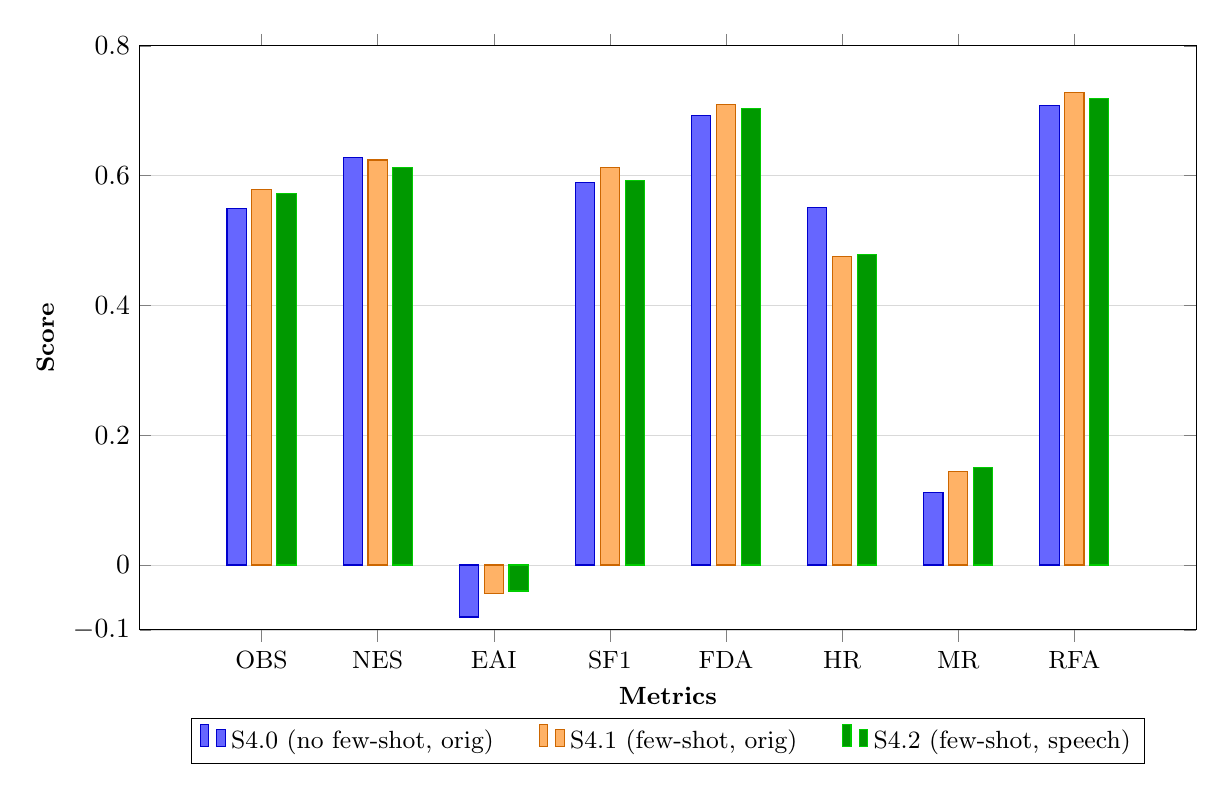
\begin{tikzpicture}
  \begin{axis}[
    width=15cm,
    height=9cm,
    ybar,
    bar width=7pt,
    ylabel={Score},
    ylabel style={font=\small\bfseries},
    xlabel={Metrics},
    xlabel style={font=\small\bfseries},
    symbolic x coords={OBS, NES, EAI, SF1, FDA, HR, MR, RFA},
    xtick=data,
    xticklabel style={font=\small},
    ymin=-0.1,
    ymax=0.8,
    ytick={-0.1, 0, 0.2, 0.4, 0.6, 0.8},
    ymajorgrids=true,
    grid style={line width=0.3pt, draw=gray!30},
    legend style={
      at={(0.5,-0.15)},
      anchor=north,
      legend columns=3,
      font=\small,
      /tikz/every even column/.append style={column sep=0.5cm}
    },
    enlarge x limits=0.15,
  ]
  
  % S4.0 (no few-shot, orig) - Blue
  \addplot[fill=blue!60, draw=blue!80!black] coordinates {
    (OBS, 0.549)
    (NES, 0.628)
    (EAI, -0.080)
    (SF1, 0.589)
    (FDA, 0.693)
    (HR, 0.551)
    (MR, 0.112)
    (RFA, 0.708)
  };
  \addlegendentry{S4.0 (no few-shot, orig)}
  
  % S4.1 (few-shot, orig) - Orange
  \addplot[fill=orange!60, draw=orange!80!black] coordinates {
    (OBS, 0.579)
    (NES, 0.624)
    (EAI, -0.044)
    (SF1, 0.613)
    (FDA, 0.709)
    (HR, 0.476)
    (MR, 0.144)
    (RFA, 0.728)
  };
  \addlegendentry{S4.1 (few-shot, orig)}
  
  % S4.2 (few-shot, speech) - Green
  \addplot[fill=green!60!black, draw=green!80!black] coordinates {
    (OBS, 0.572)
    (NES, 0.612)
    (EAI, -0.040)
    (SF1, 0.592)
    (FDA, 0.704)
    (HR, 0.479)
    (MR, 0.150)
    (RFA, 0.719)
  };
  \addlegendentry{S4.2 (few-shot, speech)}
  
  \end{axis}
\end{tikzpicture}
\caption{Headline metrics for S4 variants on MUC-4 ($N{=}100$). Few-shot prompting (S4.1) improves most accuracy-oriented metrics (OBS, SF1, FDA, RFA) but still produces negative EAI values, indicating disagreement across models at the slot level. The speech-style variant (S4.2) performs similarly to S4.1, suggesting that per-field consensus mitigates some ASR-related noise. Overall, S4 offers strong schema adherence but also highlights how per-field aggregation can amplify model inconsistencies.}
\label{fig:s4-variants-bar}
\end{figure}



\begin{figure}[H]
\centering
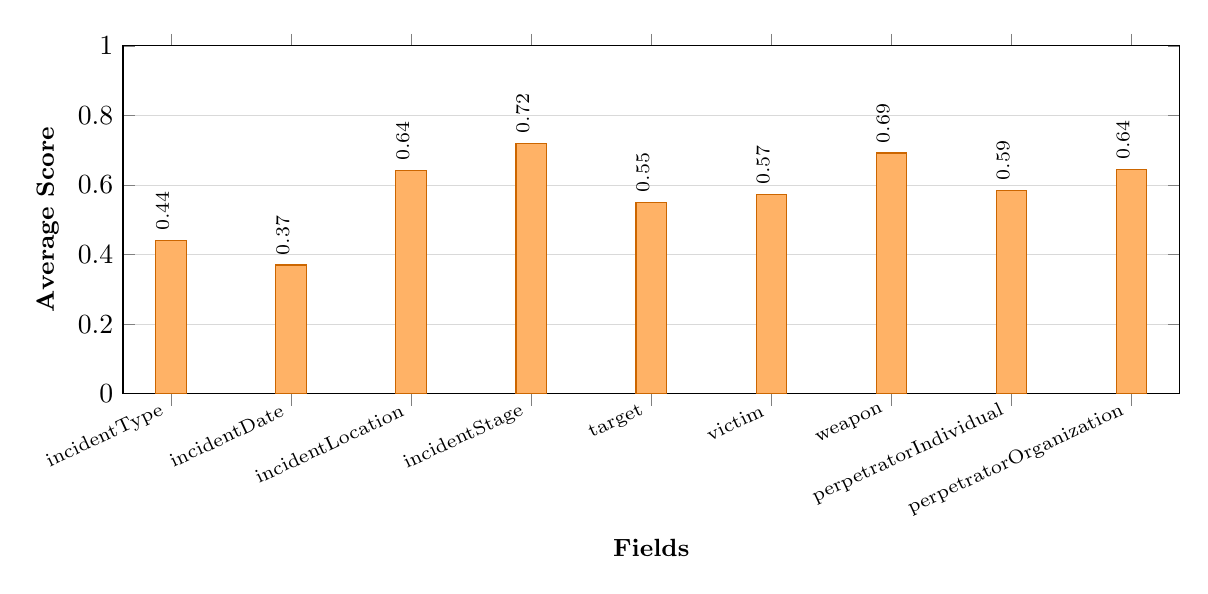
\begin{tikzpicture}
  \begin{axis}[
    width=15cm,
    height=6cm,
    ybar,
    bar width=11pt,
    ylabel={Average Score},
    ylabel style={font=\small\bfseries},
    xlabel={Fields},
    xlabel style={font=\small\bfseries},
    symbolic x coords={
      incidentType,
      incidentDate,
      incidentLocation,
      incidentStage,
      target,
      victim,
      weapon,
      perpetratorIndividual,
      perpetratorOrganization
    },
    xtick=data,
    xticklabel style={font=\scriptsize, rotate=25, anchor=east},
    ymin=0,
    ymax=1.0,
    ymajorgrids=true,
    grid style={line width=0.3pt, draw=gray!30},
    enlarge x limits=0.05,
    nodes near coords,
    nodes near coords style={
        font=\scriptsize,
        rotate=90,
        anchor=west,
        yshift=3pt
    }
  ]

  \addplot[fill=orange!60, draw=orange!80!black] coordinates {
    (incidentType, 0.440)
    (incidentDate, 0.370)
    (incidentLocation, 0.641)
    (incidentStage, 0.720)
    (target, 0.550)
    (victim, 0.572)
    (weapon, 0.692)
    (perpetratorIndividual, 0.585)
    (perpetratorOrganization, 0.644)
  };

  \end{axis}
\end{tikzpicture}
\caption{Per-field extraction performance for S4.1 on the MUC-4 subset ($N{=}100$). The per-field multi-LLM strategy performs well on structured fields such as \textit{incidentStage}, \textit{weapon}, and \textit{incidentLocation}, but struggles on more context-dependent fields like \textit{incidentType} and \textit{incidentDate}. This pattern shows how per-field consensus can stabilize well-defined slots while amplifying uncertainty in categories that require broader reasoning.}
\label{fig:s4-perfield-plot}
\end{figure}


\subsection*{Latency}

\begin{figure}[H]
\centering
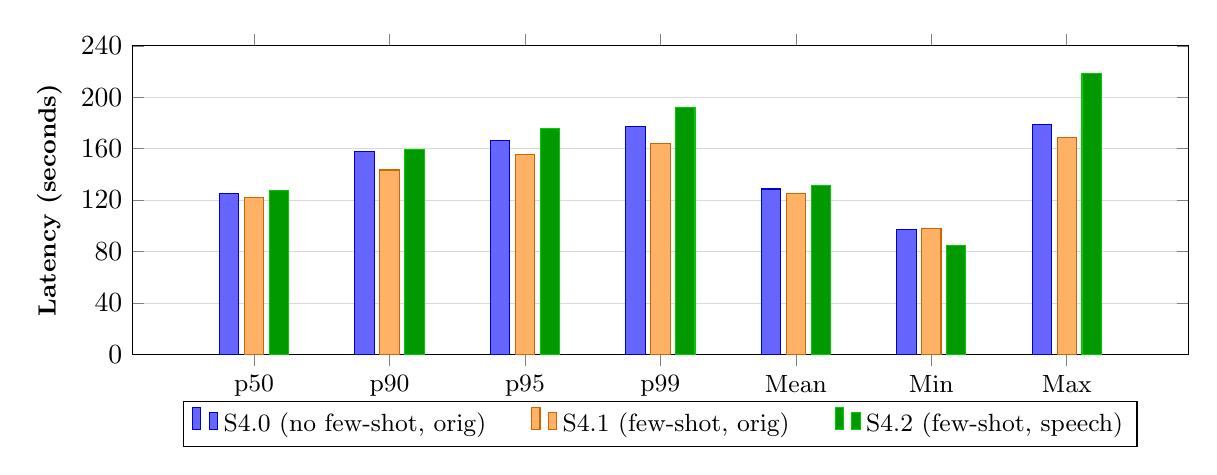
\begin{tikzpicture}
  \begin{axis}[
    width=15cm,
    height=5.5cm,
    ybar,
    bar width=7pt,
    ylabel={Latency (seconds)},
    ylabel style={font=\small\bfseries},
    xlabel={Statistics},
    xlabel style={font=\small\bfseries},
    symbolic x coords={p50, p90, p95, p99, Mean, Min, Max},
    xtick=data,
    xticklabel style={font=\small},
    ymin=0,
    ymax=240,
    ytick={0, 40, 80, 120, 160, 200, 240},
    ymajorgrids=true,
    grid style={line width=0.3pt, draw=gray!30},
    legend style={
      at={(0.5,-0.15)},
      anchor=north,
      legend columns=3,
      font=\small,
      /tikz/every even column/.append style={column sep=0.5cm}
    },
    enlarge x limits=0.15,
  ]
  
  % S4.0 (no few-shot, orig) - Blue
  \addplot[fill=blue!60, draw=blue!80!black] coordinates {
    (p50, 125.14)
    (p90, 157.96)
    (p95, 166.02)
    (p99, 177.27)
    (Mean, 128.64)
    (Min, 97.08)
    (Max, 179.00)
  };
  \addlegendentry{S4.0 (no few-shot, orig)}
  
  % S4.1 (few-shot, orig) - Orange
  \addplot[fill=orange!60, draw=orange!80!black] coordinates {
    (p50, 121.81)
    (p90, 143.39)
    (p95, 155.16)
    (p99, 164.08)
    (Mean, 124.98)
    (Min, 98.10)
    (Max, 168.81)
  };
  \addlegendentry{S4.1 (few-shot, orig)}
  
  % S4.2 (few-shot, speech) - Green
  \addplot[fill=green!60!black, draw=green!80!black] coordinates {
    (p50, 127.23)
    (p90, 159.02)
    (p95, 175.50)
    (p99, 192.16)
    (Mean, 131.15)
    (Min, 84.42)
    (Max, 218.22)
  };
  \addlegendentry{S4.2 (few-shot, speech)}
  
  \end{axis}
\end{tikzpicture}
\caption{Latency statistics for S4 variants (seconds). The per-field multi-LLM strategy shows the highest computational cost, with median latencies near 2 minutes and p99 values above 3 minutes. Few-shot prompting (S4.1) slightly lowers extreme latencies relative to S4.0, while the speech-style variant (S4.2) adds more variance. Overall, S4 highlights the trade-off between the robustness of per-field consensus and the considerable runtime required for multiple LLM calls.}
\label{fig:s4-latency-bar}
\end{figure}

Figure~\ref{fig:s4-latency-bar} makes clear that S4 is the slowest strategy family. All three variants have median latencies in the 122–127\,s range per document and heavy upper tails, with p99 values between roughly $164$\,s and $192$\,s. This behaviour is expected because S4 runs multiple models for each individual slot rather than once per document. Few-shot prompting slightly reduces median and mean latency when moving from S4.0 to S4.1, but the differences are small compared to the overall cost of per-field ensemble processing. S4.2 is marginally slower than S4.1 on average and exhibits the heaviest tail (Max above $218$\,s), reflecting additional variability in convergence on speech-style inputs. In comparison to S3.1, which also uses multi-LLM consensus but at the document level, S4 sacrifices throughput for more aggressive slot-level filling; this makes it less attractive for high-volume or time-sensitive deployments unless very high recall on nonempty fields is the primary objective.

\subsection*{Cost Analysis (S4: Multi-LLM Per-Field Consensus)}

\textbf{Assumptions.} For each of the $F{=}9$ fields, two parallel extractions are run—\textit{GPT-5} and \textit{Gemini~2.5~Pro}—with per-field averages $i_f{=}1{,}500$ input tokens and $o_f{=}50$ output tokens. A single arbiter/verification step per record runs on \textit{GPT-5-mini} with $V_{\text{in}}{=}1{,}000$ and $V_{\text{out}}{=}100$. If audio is used, Whisper transcription for $D$ minutes is added once per record.

\textbf{Prices.} GPT-5: input \$1.25/M, output \$10.00/M. Gemini~2.5~Pro: input \$1.25/M, output \$10.00/M. GPT-5-mini: input \$0.25/M, output \$2.00/M. Whisper: \$0.006/min.

\textbf{Formula.}
\[
\text{Cost}_{\text{S4}} =
\sum_{f=1}^{F}\!\Big[
\underbrace{\tfrac{i_f}{10^6}p_{\text{in}}^{(5)} + \tfrac{o_f}{10^6}p_{\text{out}}^{(5)}}_{\text{GPT-5 per field}}
+
\underbrace{\tfrac{i_f}{10^6}p_{\text{in}}^{(\text{Gemini})} + \tfrac{o_f}{10^6}p_{\text{out}}^{(\text{Gemini})}}_{\text{Gemini per field}}
\Big]
+\underbrace{\tfrac{V_{\text{in}}}{10^6}p_{\text{in}}^{(\text{mini})}+\tfrac{V_{\text{out}}}{10^6}p_{\text{out}}^{(\text{mini})}}_{\text{single arbiter}}
+0.006\cdot D
\]

\textbf{Per-record (no audio).}
\[
\begin{aligned}
\text{Per field (GPT-5): } & \tfrac{1500}{10^6}\!\cdot\!1.25 + \tfrac{50}{10^6}\!\cdot\!10.00 = \$0.002375 \\
\text{Per field (Gemini): } & \tfrac{1500}{10^6}\!\cdot\!1.25 + \tfrac{50}{10^6}\!\cdot\!10.00 = \$0.002375 \\
\text{Both models per field: } & \$0.00475 \\
\text{Across }F{=}9\text{ fields: } & 9 \times 0.00475 = \$0.04275 \\
\text{Arbiter (mini, once): } & \tfrac{1000}{10^6}\!\cdot\!0.25 + \tfrac{100}{10^6}\!\cdot\!2.00 = \$0.00045 \\
\textbf{Total: } & \mathbf{\$0.04320}\ (\approx 4.32\text{¢/doc})
\end{aligned}
\]

\textbf{With audio (Whisper).} Adding Whisper introduces a linear term $0.006\cdot D$. For $D{=}1$\,min, the total cost becomes $\$0.04320 + 0.006 = \mathbf{\$0.04920}$ (approximately $4.92$\,¢ per document). At these settings, S4 costs about $6\times$ as much as S1 (\$0.04320 vs.\ \$0.00720 per document, no audio) and roughly $2\times$ as much as S2 (\$0.04320 vs.\ \$0.02183), with the main driver being the per-field dual-model passes; the single-record arbiter remains a relatively minor component of the overall cost.

\subsection*{Consistency (Formatting \& Style)}

Figure~\ref{fig:s4-consistency} shows that S4 maintains reasonably high structural and stylistic consistency despite its aggressive fill behaviour. All variants achieve $\mathrm{FPR}_{\text{overall}}$ above $0.87$, and few-shot prompting again helps: S4.1 and S4.2 reach $0.94$, closing most of the gap to the best-performing strategies in this regard. Style-aware consistency $\mathrm{SC}_{\text{macro}}$ increases from $0.6599$ in S4.0 to $0.6881$ in S4.1, with a small drop to $0.6815$ for S4.2 on speech-style input. This suggests that the combination of per-slot prompting and consensus does not destabilise output formatting, even though the model ensemble is more willing to produce content in marginal cases.

Taken together, the S4 results characterise multi-LLM per-field consensus as an aggressive, recall-oriented strategy. It achieves high NES and strong performance on genuinely nonempty slots, particularly for context-sensitive fields such as \texttt{incidentLocation}, but this comes at the cost of elevated hallucination rates, negative EAI, and substantially higher latency and monetary cost. Compared to full-document consensus (S3.1), S4.1 offers higher NES (0.624 vs.\ 0.521) but lower OBS (0.579 vs.\ 0.641) because it overfills when gold is empty. In scenarios where maximising content recall on nonempty slots is critical and throughput is less of a concern, S4.1 is a compelling option—especially if combined with downstream post-filters. For more balanced deployments that must trade off accuracy, calibration, latency, and cost, S3.1 provides a more favourable operating point than S4’s per-field ensemble.```

\begin{figure}[H]
\centering
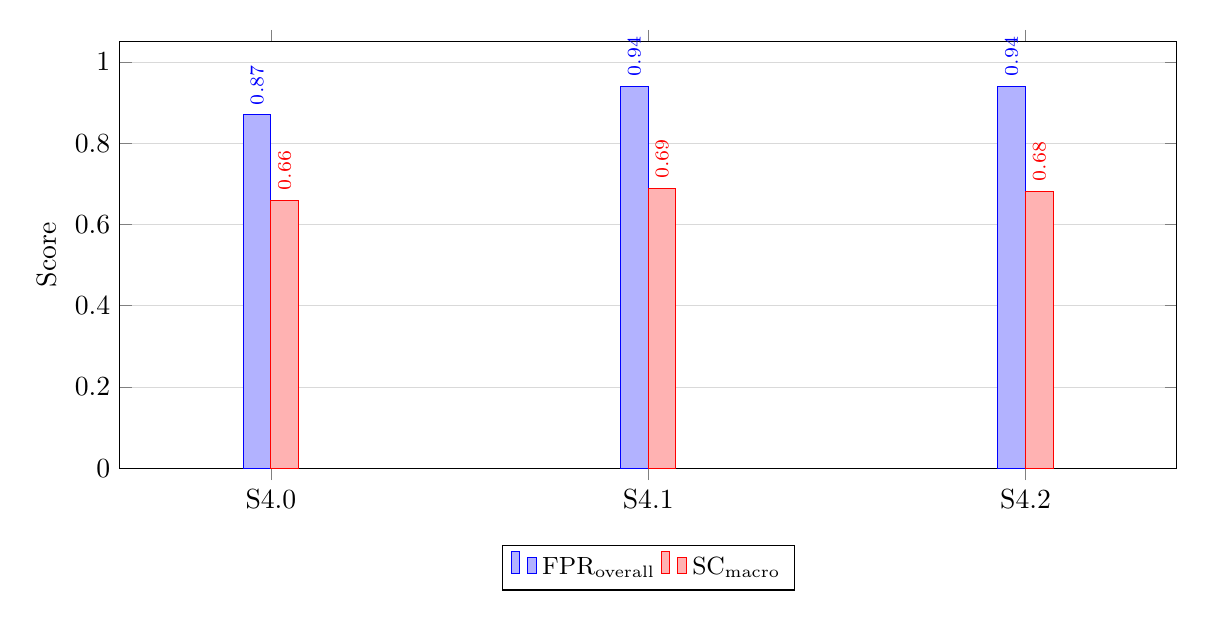
\begin{tikzpicture}
  \begin{axis}[
    width=15cm,
    height=7cm,
    ybar=0pt,
    bar width=10pt,
    ymin=0, ymax=1.05,
    ylabel={Score},
    symbolic x coords={S4.0,S4.1,S4.2},
    xtick=data,
    ymajorgrids=true,
    grid style={line width=0.3pt, draw=gray!30},
    legend style={at={(0.5,-0.18)}, anchor=north, legend columns=2, font=\small},
    enlarge x limits=0.20,
    nodes near coords,
    nodes near coords style={
        font=\scriptsize,
        rotate=90,     % vertical text
        anchor=west,
    }
  ]
    % FPR_overall
    \addplot coordinates {(S4.0,0.870) (S4.1,0.940) (S4.2,0.940)};
    \addlegendentry{$\mathrm{FPR}_{\text{overall}}$}

    % SC_macro
    \addplot coordinates {(S4.0,0.6599) (S4.1,0.6881) (S4.2,0.6815)};
    \addlegendentry{$\mathrm{SC}_{\text{macro}}$}
  \end{axis}
\end{tikzpicture}
\caption{Consistency (S4 variants): schema formatting vs.\ input-aware style.}
\label{fig:s4-consistency}
\end{figure}


\section{Comparative Analysis of Strategies}
\label{sec:eval-comparative}

This section compares the four Invox strategies (S1, S2, S3, S4) on the same dataset to identify their relative strengths and trade-offs. All results use few-shot prompting on the original MUC-4 test set (N=100).

\subsection*{Accuracy Comparison}

Figure~\ref{fig:strategy-comparison-bar} shows the main performance metrics. S1.1 reaches the highest OBS (0.644) and SF1 (0.642), with low hallucination (HR = 0.180). S4.1 has the highest NES (0.624), meaning it performs best when gold values exist, but its HR is much higher (0.476), indicating it often fills empty fields incorrectly. S2.1 and S3.1 fall between these extremes. The Empty Advantage Index (EAI) shows how much each strategy benefits from correctly leaving fields empty: S1.1 has EAI = 0.140, while S4.1 has negative EAI (-0.044), confirming it relies on filling rather than abstaining.
\begin{figure}[H]
\centering
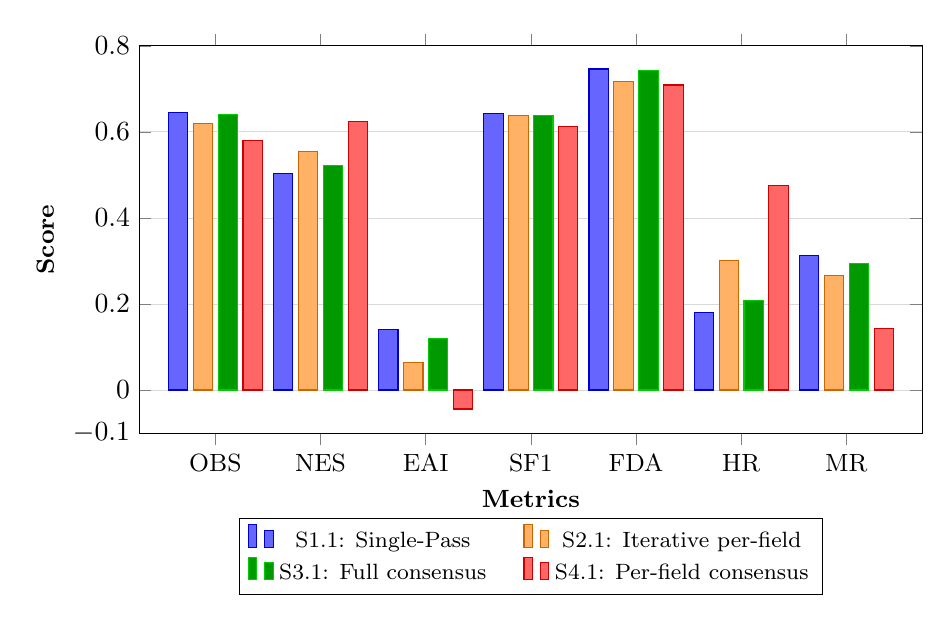
\begin{tikzpicture}
  \begin{axis}[
    width=0.95\textwidth,
    height=6.5cm,
    ybar,
    bar width=7pt,
    ylabel={Score},
    ylabel style={font=\small\bfseries},
    xlabel={Metrics},
    xlabel style={font=\small\bfseries},
    symbolic x coords={OBS, NES, EAI, SF1, FDA, HR, MR},
    xtick=data,
    xticklabel style={font=\small},
    ymin=-0.1,
    ymax=0.8,
    ytick={-0.1, 0, 0.2, 0.4, 0.6, 0.8},
    ymajorgrids=true,
    grid style={line width=0.3pt, draw=gray!30},
    legend style={
      at={(0.5,-0.22)},
      anchor=north,
      legend columns=2,
      font=\footnotesize,
      /tikz/every even column/.append style={column sep=0.4cm}
    },
    enlarge x limits=0.12,
  ]
  
  % S1.1: Single-Pass - Blue
  \addplot[fill=blue!60, draw=blue!80!black] coordinates {
    (OBS, 0.644) (NES, 0.504) (EAI, 0.140) (SF1, 0.642)
    (FDA, 0.746) (HR, 0.180) (MR, 0.313)
  };
  \addlegendentry{S1.1: Single-Pass}
  
  % S2.1: Iterative per-field - Orange
  \addplot[fill=orange!60, draw=orange!80!black] coordinates {
    (OBS, 0.619) (NES, 0.555) (EAI, 0.064) (SF1, 0.639)
    (FDA, 0.718) (HR, 0.301) (MR, 0.267)
  };
  \addlegendentry{S2.1: Iterative per-field}
  
  % S3.1: Full consensus - Green
  \addplot[fill=green!60!black, draw=green!80!black] coordinates {
    (OBS, 0.641) (NES, 0.521) (EAI, 0.120) (SF1, 0.638)
    (FDA, 0.743) (HR, 0.208) (MR, 0.295)
  };
  \addlegendentry{S3.1: Full consensus}
  
  % S4.1: Per-field consensus - Red
  \addplot[fill=red!60, draw=red!80!black] coordinates {
    (OBS, 0.579) (NES, 0.624) (EAI, -0.044) (SF1, 0.613)
    (FDA, 0.709) (HR, 0.476) (MR, 0.144)
  };
  \addlegendentry{S4.1: Per-field consensus}
  
  \end{axis}
\end{tikzpicture}
\caption{Performance comparison across four strategies (few-shot, orig MUC-4).}
\label{fig:strategy-comparison-bar}
\end{figure}


\subsection*{Cost Comparison}

Figure~\ref{fig:cost-trend-audio} shows how cost increases with audio duration. All strategies add \$0.006 per minute for Whisper transcription. The base LLM cost varies: S1.1 costs 0.72\textcent, S3.1 costs 1.40\textcent, S2.1 costs 2.18\textcent, and S4.1 costs 4.32\textcent per document (without audio). At 1 minute of audio, S4.1 is 3.7$\times$ more expensive than S1.1.
\begin{figure}[H]
\centering
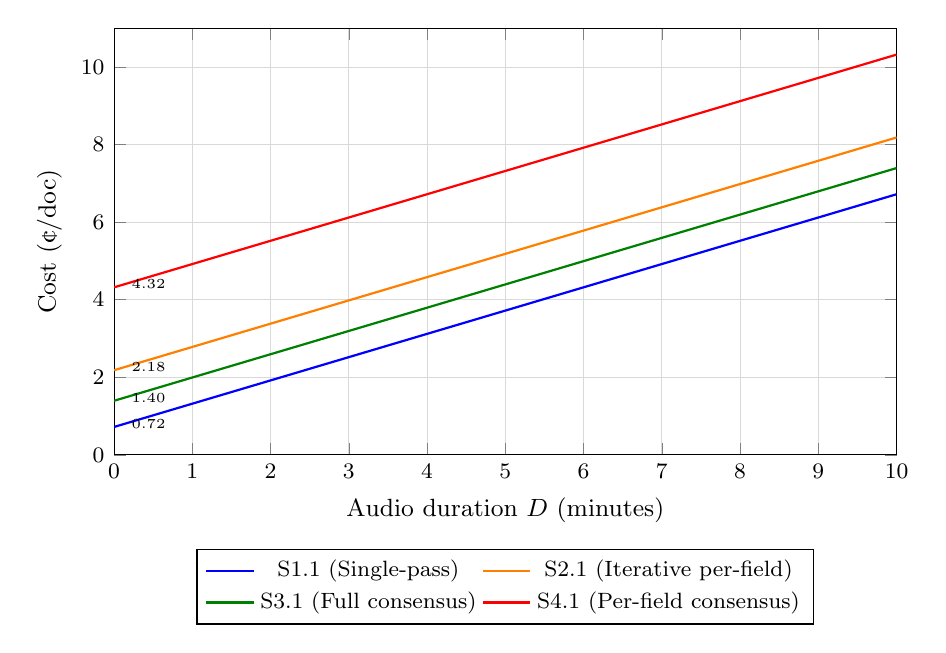
\begin{tikzpicture}
  \begin{axis}[
    width=0.95\textwidth, 
    height=7cm,
    xlabel={Audio duration $D$ (minutes)},
    ylabel={Cost (\textcent/doc)},
    xlabel style={font=\small},
    ylabel style={font=\small},
    xmin=0, xmax=10,
    ymin=0, ymax=11,
    grid=both,
    grid style={line width=0.3pt, draw=gray!30},
    legend style={at={(0.5,-0.22)}, anchor=north, legend columns=2, font=\footnotesize},
    domain=0:10,
    samples=2,
    tick label style={font=\footnotesize},
  ]

  % Removed "mark=*" from all lines
  \addplot+[thick, no markers, color=blue]  {0.72  + 0.60*x};
  \addlegendentry{S1.1 (Single-pass)}

  \addplot+[thick, no markers, color=orange] {2.183 + 0.60*x};
  \addlegendentry{S2.1 (Iterative per-field)}

  \addplot+[thick, no markers, color=green!50!black] {1.395 + 0.60*x};
  \addlegendentry{S3.1 (Full consensus)}

  \addplot+[thick, no markers, color=red] {4.32  + 0.60*x};
  \addlegendentry{S4.1 (Per-field consensus)}

  % Baseline labels
  \node[anchor=west, font=\tiny] at (axis cs:0.1,0.80) {0.72};
  \node[anchor=west, font=\tiny] at (axis cs:0.1,2.26) {2.18};
  \node[anchor=west, font=\tiny] at (axis cs:0.1,1.47) {1.40};
  \node[anchor=west, font=\tiny] at (axis cs:0.1,4.40) {4.32};

  \end{axis}
\end{tikzpicture}
\caption{Cost vs.\ audio duration: $\text{cost}(D)=\text{base}+0.60D$ (\textcent/doc).}
\label{fig:cost-trend-audio}
\end{figure}


\subsection*{Latency Comparison}


\begin{figure}[H]
\centering
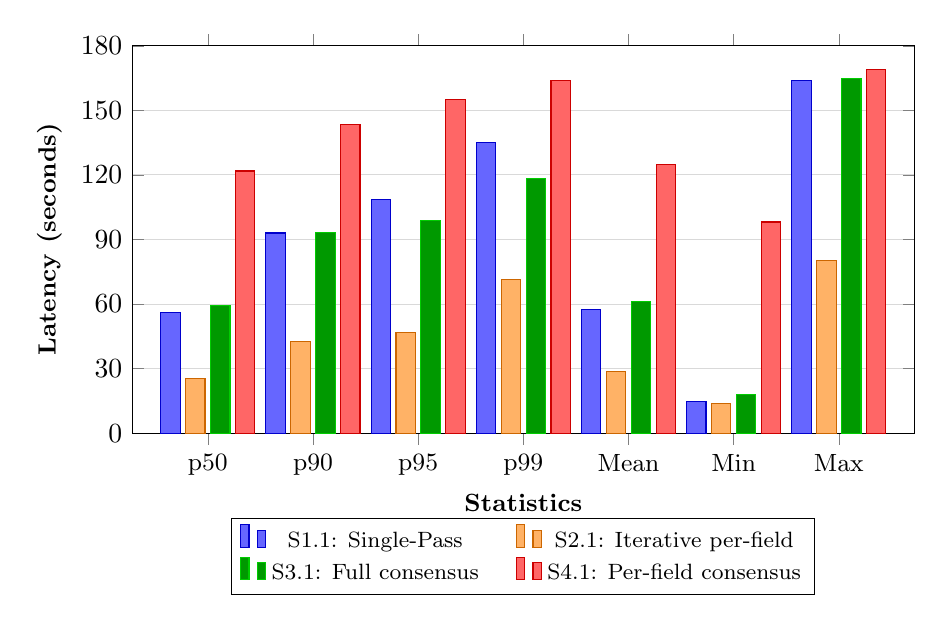
\begin{tikzpicture}
  \begin{axis}[
    width=0.95\textwidth,
    height=6.5cm,
    ybar,
    bar width=7pt,
    ylabel={Latency (seconds)},
    ylabel style={font=\small\bfseries},
    xlabel={Statistics},
    xlabel style={font=\small\bfseries},
    symbolic x coords={p50, p90, p95, p99, Mean, Min, Max},
    xtick=data,
    xticklabel style={font=\small},
    ymin=0,
    ymax=180,
    ytick={0, 30, 60, 90, 120, 150, 180},
    ymajorgrids=true,
    grid style={line width=0.3pt, draw=gray!30},
    legend style={
      at={(0.5,-0.22)},
      anchor=north,
      legend columns=2,
      font=\footnotesize,
      /tikz/every even column/.append style={column sep=0.4cm}
    },
    enlarge x limits=0.12,
  ]
  
  % S1.1: Single-Pass - Blue
  \addplot[fill=blue!60, draw=blue!80!black] coordinates {
    (p50, 55.91) (p90, 93.01) (p95, 108.40) (p99, 134.93)
    (Mean, 57.34) (Min, 14.54) (Max, 163.79)
  };
  \addlegendentry{S1.1: Single-Pass}
  
  % S2.1: Iterative per-field - Orange
  \addplot[fill=orange!60, draw=orange!80!black] coordinates {
    (p50, 25.35) (p90, 42.48) (p95, 46.68) (p99, 71.52)
    (Mean, 28.58) (Min, 13.60) (Max, 80.28)
  };
  \addlegendentry{S2.1: Iterative per-field}
  
  % S3.1: Full consensus - Green
  \addplot[fill=green!60!black, draw=green!80!black] coordinates {
    (p50, 59.39) (p90, 93.15) (p95, 98.77) (p99, 118.28)
    (Mean, 61.09) (Min, 18.13) (Max, 164.96)
  };
  \addlegendentry{S3.1: Full consensus}
  
  % S4.1: Per-field consensus - Red
  \addplot[fill=red!60, draw=red!80!black] coordinates {
    (p50, 121.81) (p90, 143.39) (p95, 155.16) (p99, 164.08)
    (Mean, 124.98) (Min, 98.10) (Max, 168.81)
  };
  \addlegendentry{S4.1: Per-field consensus}
  
  \end{axis}
\end{tikzpicture}
\caption{Latency distribution across strategies (seconds).}
\label{fig:latency-comparison-bar}
\end{figure}



\subsection*{Consistency Comparison}

Figure~\ref{fig:consistency-cross-strategy} compares how well each strategy follows the schema format (FPR$_{\text{overall}}$) and maintains consistent writing style (SC$_{\text{macro}}$). The baseline S5 (LangExtract) has perfect format compliance (1.000) because it uses strict validation rules. Among Invox strategies, S1.1 has the highest format score (0.960). For style consistency, S1.1 and S3.1 both reach 0.724, slightly higher than S2.1 (0.683) and S4.1 (0.688).

\begin{figure}[H]
\centering
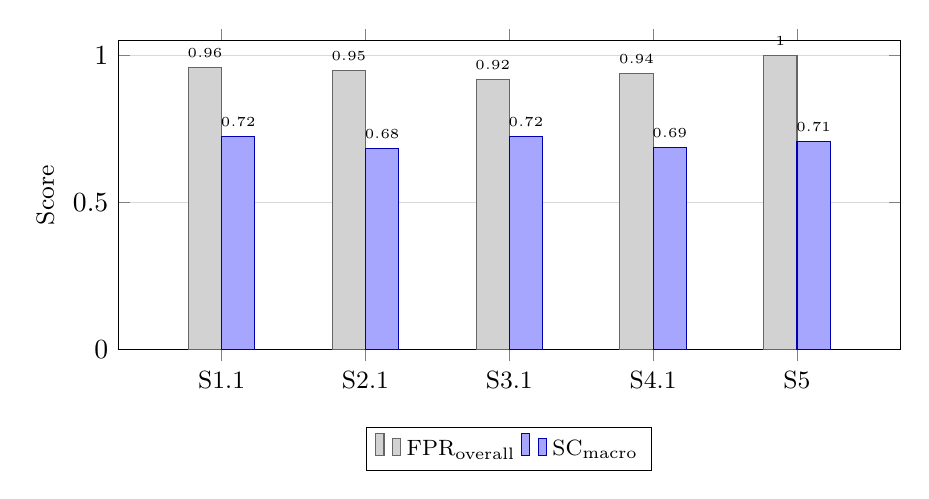
\begin{tikzpicture}
  \begin{axis}[
    width=0.95\textwidth,
    height=5.5cm,
    ybar=0pt,
    bar width=12pt,
    ymin=0, ymax=1.05,
    ylabel={Score},
    ylabel style={font=\small},
    symbolic x coords={S1.1,S2.1,S3.1,S4.1,S5},
    xtick=data,
    xticklabel style={font=\small},
    ymajorgrids=true,
    grid style={line width=0.3pt, draw=gray!30},
    legend style={at={(0.5,-0.25)}, anchor=north, legend columns=2, font=\footnotesize},
    enlarge x limits=0.18,
    nodes near coords,
    nodes near coords style={font=\tiny},
    nodes near coords align={vertical},
  ]
    \addplot[fill=gray!35, draw=black!60] coordinates {
      (S1.1,0.960) (S2.1,0.950) (S3.1,0.920) (S4.1,0.940) (S5,1.000)
    };
    \addlegendentry{$\mathrm{FPR}_{\text{overall}}$}

    \addplot[fill=blue!35, draw=blue!70!black] coordinates {
      (S1.1,0.724) (S2.1,0.683) (S3.1,0.724) (S4.1,0.688) (S5,0.709)
    };
    \addlegendentry{$\mathrm{SC}_{\text{macro}}$}
  \end{axis}
\end{tikzpicture}
\caption{Format compliance and style consistency across strategies.}
\label{fig:consistency-cross-strategy}
\end{figure}


\subsection*{Observed Trade-offs}

The four strategies show clear patterns:

\textbf{S1.1 (Single-LLM Full-Input)} achieves the best overall scores (OBS = 0.644), balancing accuracy, speed (median 55.91s), cost (0.72\textcent), and lowest hallucination (0.180).

\textbf{S2.1 (Single-LLM One-Field)} is fastest (median 25.35s) through parallel processing. Accuracy is slightly lower (OBS = 0.619) with higher hallucination (0.301), but improves location fields.

\textbf{S3.1 (Multi-LLM Full-Input)} runs two models, reducing hallucination (HR = 0.208) and improving NES (0.521 vs.\ 0.504). Speed and cost fall between S1.1 and S2.1.

\textbf{S4.1 (Multi-LLM One-Field)} runs two models per field, achieving highest NES (0.624) and lowest missing rate (0.144), but highest hallucination (0.476). It is slowest (median 121.81s) and most expensive (4.32\textcent).

The main trade-off is filling correctly when values exist (NES, MR) versus abstaining when absent (HR, EAI). S1.1 and S3.1 balance both. S2.1 prioritizes speed. S4.1 prioritizes recall over precision.



\chapter{Conclusion}
\label{chap:conclusion}
This chapter summarizes the contributions of this thesis, highlights key findings, discusses limitations, and outlines implications for practice. The goal of the thesis was to design and implement a privacy-preserving vulnerability detection and repair assistant for Visual Studio Code that leverages locally deployed LLMs and retrieval-augmented grounding without transmitting source code to external services.

\section{Summary of Contributions}

\textbf{Code Guardian: an IDE-integrated, local security assistant.}
This thesis delivers \textbf{Code Guardian}, a VS Code extension that performs on-device vulnerability analysis for JavaScript and TypeScript projects. Findings are presented using IDE-native diagnostics, and optional quick fixes provide repair suggestions while keeping developers in full control of code changes.

\textbf{Privacy-preserving LLM inference with optional RAG.}
All code analysis runs locally via Ollama. To improve grounding, the system optionally augments prompts with locally retrieved security knowledge (CWE/OWASP/CVE guidance) using a local vector index and local embeddings. This architecture supports explainability and consistency while preserving the no-exfiltration requirement.

\textbf{Practical performance mechanisms.}
To remain usable during development, Code Guardian combines debounced triggers, function-level scoping for real-time use, and caching of repeated analyses. These mechanisms reduce unnecessary inference calls and support responsive IDE feedback.

\textbf{Reproducible evaluation harness.}
The prototype includes a curated benchmark of security test cases and a local evaluation script for comparing models and configurations using standard detection metrics, parse robustness, and latency.

\section{Limitations}

\textbf{Scope limits and contextual depth.}
While the system can flag common vulnerability patterns, deep semantic reasoning across files (e.g., source-to-sink flows spanning modules) is limited by the analysis scope and the absence of full static data-flow analysis.

\textbf{Evaluation representativeness.}
The curated dataset is intentionally small and human-auditable, but it does not fully reflect the diversity and ambiguity of real-world codebases. Results should therefore be interpreted as indicative rather than definitive.

\textbf{Repair correctness.}
Repair suggestions are model-generated and may affect behavior beyond security hardening. The system mitigates this by requiring explicit user review, but comprehensive functional validation remains outside the scope of the extension.

\section{Conclusion}

Privacy-preserving secure coding assistance is feasible within the IDE when local LLM inference is combined with careful prompt structuring, optional retrieval grounding, and developer-controlled remediation workflows. Code Guardian demonstrates that locally deployed LLMs can provide actionable vulnerability detection and repair suggestions without transmitting source code off-device, while remaining compatible with interactive development constraints.


\chapter{Future Work}
\label{chap:future-work}
Building on the contributions and limitations above, several next steps stand out for improving Code Guardian’s effectiveness, robustness, and evaluation depth.

\noindent\textbf{Deeper program analysis and cross-file context.}
Add lightweight static analysis to extract taint-style source-to-sink traces across functions and files, and feed these traces into the LLM prompt. This can reduce false positives from missing context and improve recall for vulnerabilities that span modules (e.g., validation in one file and sink usage in another).

\medskip

\noindent\textbf{Hybrid integration with traditional SAST.}
Integrate rule-based baselines (e.g., Semgrep) as an additional signal. A hybrid approach can use SAST findings as candidate locations and let the LLM focus on contextual reasoning and repair generation, improving both precision and developer trust.

\medskip

\noindent\textbf{Repair validation and safer patching.}
Extend repair suggestions with syntactic checks and minimal local validation (e.g., TypeScript typechecking on modified regions). Provide diff previews by default and track when suggested fixes introduce new warnings.

\medskip

\noindent\textbf{Adversarial robustness.}
Study prompt-injection and retrieval-poisoning risks within the IDE context (e.g., attacker-controlled comments or dependency code). Add provenance and filtering for retrieved knowledge, and implement safe prompt templates that explicitly treat code as data.

\medskip

\noindent\textbf{Broader evaluation on standard benchmarks and real repositories.}
Complement the curated dataset with larger benchmarks (e.g., OWASP Benchmark, Juliet-style suites) and selected real-world CVE cases. Report confidence intervals, paired significance tests (e.g., McNemar/permutation on per-sample outcomes), and per-category breakdowns, and compare against SAST baselines under matched conditions.

\medskip

\noindent\textbf{User studies in realistic IDE workflows.}
Run a developer study to measure time-to-fix, perceived usefulness, trust calibration, and false-positive tolerance. Standard usability and workload instruments such as SUS and NASA-TLX can complement objective metrics \cite{brooke1996sus,hart1988nasa}. Compare LLM-only vs.\ LLM+RAG configurations under real editing sessions to validate R6 and practical adoption constraints.


% =======================
% APPENDICES GO HERE
% =======================
\appendix


\chapter{Detailed Implementation Results}
\label{appendix:detailed-implementation}
\section{Consistency Formatting (CF) Agent}
\label{app:cf-impl}

Listing~\ref{lst:cf-transforms} shows the main helper functions used by the CF agent for deterministic normalization. These correspond to the transformation rules described in Section~\ref{subsec:impl-cf}.

\begin{lstlisting}[language=Java, caption={CF agent transformation function signatures}, label={lst:cf-transforms}]
function normalizeDate(value: string): string | null;

function normalizeNumber(value: string): number | null;

function validateEnum(v: string, o: string[]): string | null;

function joinMultiValue(values: any[]): string | null;

function normalizeText(value: string): string | null;
\end{lstlisting}

\section{IE Agent Supporting Types}
\label{appendix:detailed-implementation}

Listing~\ref{lst:ie-types} defines the supporting types used by the IE agent to represent current and filled field values.

\begin{lstlisting}[language=Java, caption={Supporting types for the IE agent}, label={lst:ie-types}]
interface CurrentFieldValue {
  value: any;
  locked?: boolean;             
  source?: "ai" | "manual";     
}

interface FilledField {
  value: any;
  changed: boolean;             
  previousValue?: any;          
  source: "ai" | "manual";
  confidence?: number;         
}
\end{lstlisting}

\section{Verification Agent API}
\label{app:ver-api}

Listing~\ref{lst:ver-api} provides the TypeScript interfaces for the verification agent, as described conceptually in Section~\ref{subsec:impl-ver}.

\begin{lstlisting}[language=Java, caption={Verification agent API contract}, label={lst:ver-api}]
interface VerificationInput {
  cand: Record<string, FilledField> | Record<string, FilledField>[];
  transcript: string;           
  fields: FormTemplateField[];
  currentValues?: Record<string, CurrentFieldValue>;
}

interface VerificationOutput {
  filled: Record<string, FilledField>;
  confidence: Record<string, number>;  
  issues?: Array<{
    field: string;
    type: "missing" | "conflict" | "low_conf" | "invalid";
    detail: string;
    action?: "requery" | "clarify" | "manual_review";
  }>;
  decisions?: Array<{             
    field: string;
    decision: "gpt" | "gemini" | "merge" | "keep_current";
    reason: string;
  }>;
}
\end{lstlisting}

\section{Orchestrator Implementation}
\label{app:orchestrator-impl}

Listing~\ref{lst:orchestrator-core} presents the core orchestration logic as implemented in the \texttt{Orchestrator} class. This corresponds to the conceptual pipeline described in Section~\ref{subsec:impl-orchestration}.

\begin{lstlisting}[language=Java, caption={Core orchestration logic of the Invox pipeline}, label={lst:orchestrator-core}]
class Orchestrator {
  async processTemplate(in: ProcessingRequest): Promise<FinalTemplate> {
    // Step 1: Transcription (optional)
    const transcript = in.audio 
      ? await stt.transcribe(in.audio)
      : { transcript: in.text, language: in.lang ?? "en" };

    // Step 2: Retrieval (RAG)
    const examples = await rag.retrieve(
      transcript.transcript,
      in.fields,
      in.templateId
    );

    // Step 3: Extraction (strategy-dependent)
    const extraction = await this.runStrategy({
      strategy: in.strategy,
      transcript: transcript.transcript,
      fields: in.fields,
      currentValues: in.currentValues,
      fewShots: examples.examples,
      ...in.metadata,
    });

    // Step 4: Formatting (deterministic normalization)
    const norm = await cf.normalize(extraction.filled, in.fields);

    // Step 5: Verification (completeness + consistency)
    const verified = await ver.verify({
      candidates: norm,
      transcript: transcript.transcript,
      fields: in.fields,
      currentValues: in.currentValues,
    });

    // Step 6: Clarification loop (if needed)
    if (verified.issues?.some(i => i.action === "requery")) {
      // Re-run IE with hints from VER, then re-verify
    }

    return {
      filled: verified.filled,
      confidence: verified.confidence,
      issues: verified.issues,
      model: extraction.model,
      transcript: transcript.transcript,
    };
  }

  private async runStrategy(p: StrategyParams): Promise<IEOutput> {
    switch (p.strategy) {
      case "S1": return await singleLlmAllField(p);
      case "S2": return await singleLlmOneField(p);
      case "S3": return await dualLlmAllField(p);
      case "S4": return await multiLlmOneField(p);
    }
  }
}
\end{lstlisting}


\section{Strategy Function Implementations}
\label{app:strategy-impl}

This section provides simplified TypeScript sketches of the four strategy functions and the strategy-level orchestrator described in Section~\ref{sec:impl-strategies}. The listings are not intended as production-ready code, but as an executable illustration of the control flow.

\subsection*{S1: \texttt{singleLlmAllField}}

\begin{lstlisting}[language=Java, caption={Core S1 implementation sketch (\texttt{singleLlmAllField})}, label={lst:s1-impl}]
export async function singleLlmAllField(
  input: GetFilledTemplateInput
): Promise<GetFilledTemplateResult> {
  const {
    oldText,
    newText,
    fields,
    currentValues,
    modelName,
    transcriptData,
  } = input;

  // 1. Combine transcripts
  const combTrans = oldText ? `${oldText}\n${newText}` : newText;
  
  // 2. Retrieve few-shot examples
  const fewShots = await getFewShotsFromTranscript(
    combinedTranscript,
    fields,
    3
  );
  
  // 3. Single LLM call for all fields
  const schema = z.object(/* comprehensive field schema */);
  const result = await generateObject({
    model: openai(modelName),
    schema,
    prompt: buildComprehensivePrompt(
      fields,
      oldText,
      newText,
      fewShots
    ),
  });
  
  // 4. Process results
  const filled = processAllFields(
    result.object,
    fields,
    currentValues
  );
  const verified = await runVerifier(
    combTrans,
    fields,
    filled
  );
  
  return {
    filled: verified,
    model: modelName,
    transcript: transcriptData,
  };
}
\end{lstlisting}

\subsection*{S2: \texttt{singleLlmOneField}}

\begin{lstlisting}[language=Java, caption={Core S2 implementation sketch (\texttt{singleLlmOneField})}, label={lst:s2-impl}]
export async function singleLlmOneField(
  input: GetFilledTemplateInput
): Promise<GetFilledTemplateResult> {
  const {
    oldText,
    newText,
    fields,
    currentValues,
    modelName,
    transcriptData,
  } = input;

  const combTrans = oldText ? `${oldText}\n${newText}` : newText;

  // Retrieve few-shot examples once
  const fewShots = await getFewShotsFromTranscript(
    combTrans,
    fields,
    3
  );
  
  // Parallel field processing with individual error boundaries
  const tasks = fields.map(field =>
    runField({
      field,
      oldText,
      newText,
      fewShots,
      current: currentValues?.[field.id],
      modelName,
    }).catch(error => {
      // Field-level error recovery
      return [field.id, getFallbackField(field, currentValues)];
    })
  );
  
  const entries = await Promise.all(tasks);

  return {
    filled: Object.fromEntries(entries),
    model: modelName,
    transcript: transcriptData,
  };
}
\end{lstlisting}

\subsection*{S3: \texttt{dualLlmAllField}}

\begin{lstlisting}[language=Java, caption={Core S3 implementation sketch (\texttt{dualLlmAllField})}, label={lst:s3-impl}]
export async function dualLlmAllField(
  input: GetFilledTemplateInput
): Promise<GetFilledTemplateResult> {
  const {
    oldText,
    newText,
    fields,
    currentValues,
    gptModel,
    geminiModel,
    transcriptData,
  } = input;

  const combTrans = oldText ? `${oldText}\n${newText}` : newText;
  const fewShots = await getFewShotsFromTranscript(
    combTrans,
    fields,
    3
  );

  const schema = z.object(/* comprehensive field schema */);
  const prompt = buildComprehensivePrompt(
    fields,
    oldText,
    newText,
    fewShots
  );

  // Parallel model execution
  const [gptResult, geminiResult] = await Promise.all([
    generateObject({ model: openai(gptModel), schema, prompt }),
    generateObject({ model: google(geminiModel), schema, prompt }),
  ]);
  
  // Build candidates
  const gptCandidate = buildCandidate(
    gptResult.object,
    fields,
    currentValues
  );
  const geminiCandidate = buildCandidate(
    geminiResult.object,
    fields,
    currentValues
  );

  // Consensus verification
  const verified = await runEnsembleVerifier({
    combTrans,
    fields,
    currentValues,
    gpt: gptCandidate,
    gemini: geminiCandidate,
  });
  
  return {
    filled: verified.filled,
    model: `ensemble:${gptModel}+${geminiModel}`,
    transcript: transcriptData,
  };
}
\end{lstlisting}

\subsection*{S4: \texttt{multiLlmOneField}}

\begin{lstlisting}[language=Java, caption={Core S4 implementation sketch (\texttt{multiLlmOneField})}, label={lst:s4-impl}]
export async function multiLlmOneField(
  input: GetFilledTemplateInput
): Promise<GetFilledTemplateResult> {
  const {
    oldText,
    newText,
    fields,
    currentValues,
    gptModel,
    geminiModel,
    verifierModel,
    transcriptData,
  } = input;

  const combTrans = oldText ? `${oldText}\n${newText}` : newText;
  const fewShots = await getFewShotsFromTranscript(
    combTrans,
    fields,
    3
  );

  const results: [string, FilledField][] = [];
  
  // Sequential field processing (rate limit avoidance)
  for (const field of fields) {
    const entry = await runOneFieldWithEnsemble({
      field,
      oldText,
      newText,
      fewShots,
      current: currentValues?.[field.id],
      gptModel,
      geminiModel,
      verifierModel,
    });
    results.push(entry);
  }
  
  return {
    filled: Object.fromEntries(results),
    model: `ensemble-per-field:${gptModel}+${geminiModel}`,
    transcript: transcriptData,
  };
}
\end{lstlisting}

\subsection*{\texttt{StrategyOrchestrator} Sketch}

\begin{lstlisting}[language=Java, caption={Strategy-level orchestrator sketch}, label={lst:strategy-orchestrator}]
class StrategyOrchestrator {
  constructor(
    private readonly singlePass: SinglePassStrategy,
    private readonly iterative: IterativeStrategy,
    private readonly multiModelFull: MultiModelFullStrategy,
    private readonly multiModelSlot: MultiModelSlotStrategy
  ) {}

  async executeStrategy(
    input: ProcessingRequest
  ): Promise<FinalTemplate> {
    const impl = this.getStrategyImplementation(input.strategy);
    return await impl.execute(input);
  }
  
  private getStrategyImplementation(
    strategy: Strategy
  ): StrategyImplementation {
    switch (strategy) {
      case "S1":
        return this.singlePass;
      case "S2":
        return this.iterative;
      case "S3":
        return this.multiModelFull;
      case "S4":
        return this.multiModelSlot;
      default:
        throw new Error(`Unknown strategy: ${strategy}`);
    }
  }
}
\end{lstlisting}


\chapter{Detailed Experimental Results}
\label{appendix:detailed-results}
\section{Curated Test Suite Overview}
\label{app:dataset-overview}

The curated evaluation suite maintained in \texttt{code-guardian/evaluation/datasets/} contains representative vulnerability snippets for JavaScript/TypeScript secure coding. Expected vulnerabilities include CWE identifiers and severities so results can be aggregated by category.

\subsection*{Dataset sizes}

At the time of writing, the suite contains:
\begin{itemize}
  \item \textbf{Core dataset:} 20 test cases (18 vulnerable, 2 secure)
  \item \textbf{Advanced dataset:} 28 test cases (25 vulnerable, 3 secure)
\end{itemize}
The repository-contained evaluation harness loads the core dataset by default; the advanced dataset is included to broaden coverage and can be evaluated by extending the harness.

\subsection*{Representative Vulnerability Classes}

The dataset includes (non-exhaustive) examples for:
\begin{itemize}
  \item SQL injection (CWE-89)
  \item Cross-site scripting (CWE-79)
  \item Command injection (CWE-78)
  \item Path traversal (CWE-22)
  \item Insecure randomness (CWE-330)
  \item Hardcoded credentials (CWE-798)
  \item Insecure CORS / CSRF patterns (CWE-352 and related)
\end{itemize}

\subsection*{Test Case Record Format}

Each test case contains:
\begin{itemize}
  \item a code snippet (\texttt{code}),
  \item a list of expected findings (\texttt{expectedVulnerabilities}),
  \item and optional remediation guidance (\texttt{expectedFix}).
\end{itemize}

\subsection*{Reproducing the harness run}

The evaluation script is executed locally:
\begin{lstlisting}[language=Java, caption={Running the evaluation script}, label={lst:appendix-eval-run}]
cd code-guardian
node evaluation/evaluate-models.js
\end{lstlisting}

The script prints per-model precision/recall/F1, false positive rate, average response time, and JSON parse success rate. Models to test are specified in the script and can be edited to match the locally installed Ollama models.

This appendix is intentionally concise: the full dataset is machine-readable and can be inspected directly in the repository.


% =====================================================
% BACKMATTER: Bibliography, Index, etc.
% =====================================================
\backmatter

\bibliographystyle{splncs03}
\bibliography{bibliography}

\printindex

\end{document}
